\documentclass[a4paper]{article}
\usepackage{fontspec}\defaultfontfeatures{Ligatures=TeX}
% \usepackage{setspace}\setstretch{1.1} % \begin{spacing}{1.3}
\usepackage[a4paper,vmargin={4cm,4cm},hmargin={4cm,4cm}]{geometry}
%-----------------------------------------------------------------------------%
\usepackage{settings}
\usepackage{settings-biblatex}
\usepackage{settings-color}
\usepackage{settings-math}
\usepackage{settings-algorithm}
\usepackage{settings-cjk}
\usepackage{settings-gloss}
\usepackage{settings-tables}
%-----------------------------------------------------------------------------%
%%% Title %%%
\title{A Bayesian Approach\\to the Problem of Unknown Networks\\in Spatial Autoregressive Models}
\author{陳\,捷\\Jesse Chieh Chen\thanks{National Taiwan University. Contact: \url{https://jessekelighine.com}.}}
\date{Draft: \texttt{\today}}
%-----------------------------------------------------------------------------%

\begin{document}

\maketitle

\begin{abstract}
	\noindent
	We introduced a Bayesian method for estimating unknown networks in the context of \acrlong{sar} models
	by introducing a network formation model, \acrlong{ergm} in this paper, as a prior distribution.
	This method brings two main advantages:
	first, this method is a natural extension to common high-dimensional methods;
	second, this method enables the econometrician to incorporate prior knowledge or belief
	about the network formation process with great flexibility.
	Via simulation studies,
	we demonstrated this approach is practical in recovering unknown networks ties and higher-order characteristics
	of the network.
\end{abstract}

\section{Introduction}\label{sec:introduction}

\gls{sar} is one of the main methods econometrician employ to study network effects.
This approach requires the underlying network to be known to the researcher.
However, it is usually difficult to obtain network data.
For example,
if we are interested in peer effect within a certain class,
it is easy to known the pupils' individual characteristics (age, sex, GPA, etc),
but difficult to know the friendship network.
Hence it is natural to extend the canonical \gls{sar} model with known networks to the case where the network is unknown,
but is \emph{believed} to exist by the researcher.

The estimation of unknown network has been of interest for a long time.
There are interests from various disciplines
that seeks to tackle the problem of unknown network from different perspectives.
In biology, the interest are mainly focused on retrieving the covariance between different covariates
(see \cite{yuan-2007})
or recovering the \gls{dag} structure of covariates (see \cite{madigan-1994}).
These methods usually apply to relatively small number of nodes or covariates (usually no larger than 10)
and deal with structures with relatively low complexity.

Compared to the research interest from biology,
social networks to contain more nodes and more complex structures.
The interest among economists about social network mainly began with \cite{ord-1975} and later with \cite{manski-1993}.
Following it, many researchers have studied the problem of estimating the effect of social interactions
and network formation (see \cite{anselin-2009} for a survey of these results).
These methods focuses on known networks.
Recent literature seeks to tackle the problem of unknown network.
The problem is two-fold: the first is about identification, the second is about estimation.
On the identification problem,
most of the literature utilize some assumption about sparsity of the social network adjacency matrix
(e.g.\ \cite{rose-2017});
\cite{blume-2015} utilizes a \emph{partially} observed network and assumes some individual are known not to connect.
Other efforts such as \cite{bonaldi-2015} and \cite{manresa-2016}
further assume that there is no \emph{endogenous effect} \parencite{manski-1993}.

Many of these assumptions also carry through to estimation,
i.e., sparsity assumptions translates directly to penalized or regularized estimations.
For example, \cite{lam-2020} and \cite{meinshausen-2006} uses penalized methods to estimate unobserved networks.
One recent working paper \cite{de_paula-2023} identifies the unknown network \emph{without} sparsity assumptions
but still utilizes adaptive elastic net \parencite{caner-zhang-2014} in estimation.
The successful use of high-dimensional methods naturally suggests a Bayesian approach.

Bayesian inference methods are present in the literature of social networks (e.g., \cite{hsieh-2018})
along with some software support (e.g., \cite{caimo-friel-2014}).
The classical \gls{sar} model with known network can be estimated with Bayesian methods.
However, in the fields of unknown networks, Bayesian treatment is largely absent.
Recently, \cite{krisztin-piribauer-2022} also proposed a Bayesian treatment
to the problem of unknown networks in \gls{sar} models.
In their paper, they considered \gls{er} type priors.
This is, to our knowledge, the first attempt in recovering unknown networks in the context of \gls{sar} via a Bayesian methodology.

The approach presented by \cite{krisztin-piribauer-2022} is the Bayesian analogue to the frequentest high-dimensional method.
It is well known that high-dimensional methods closely relates to Bayesian methods,
and \gls{er} type priors relates directly to sparsity (as they mentioned themselves)
and only incorporates ``local'' information (dyadic).
However, Bayesian methods allows us to go beyond regularizations of simple forms,
e.g., Ridge or Lasso,
and form regularizations with economic meaning and microfoundation.
Our approach goes beyond the sparsity assumption and motivate the Bayesian approach from a network formation point of view.
This allows us to also incorporates ``global'' and ``structural'' information (e.g., mutuality, triangles) in the prior
while preserving ``sparsity.''
Thus, this paper can be viewed as an extension of \cite{krisztin-piribauer-2022}.

The rest of this paper is structured thus:
in \autoref{sec:model-setup}, the motivation and model setup are given;
in \autoref{sec:model-specifications}, the full Bayesian models are specified;
in \autoref{sec:sampling-procedure}, the procedure for posterior sampling is presented;
in \autoref{sec:simulation-study}, simulations studies are performed;
in \autoref{sec:discussion}, a discussion and conclusion is given.

\section{Model Setup}\label{sec:model-setup}

This research focuses on \gls{sar}.
The canonical \gls{sar} assumes the form
\begin{align}\label{eq:sar}
	\underset{(N\times 1)}{\yy}
	= \lambda\underset{(N\times N)}{\bar\WW}\yy
	+ \underset{(N\times K)}{\XX_{1}}\underset{(K\times 1)}{\bbeta_1}
	+ \bar\WW\XX_{2}\bbeta_2
	+ \uu
\end{align}
where $\yy$ is the vector of outcome variables (e.g., GPA of all students in a class),
$\bar\WW$ is the row-normalized adjacency matrix representation of the underlying network $\WW$ (e.g., friendship network of the class),
\footnote{
	In many studies, the network matrix is \emph{row-normalized}. (See, e.g., \cite{lesage-pace-2009})
	That is, rows of the network matrix in the \gls{sar} sums to one.
	This is usually done for two purposes:
	to make the direct effect $\lambda$ easier to interpret (as $N\to\infty$) and
	to ensure asymptotic properties of the estimators. (See, e.g., \cite{lee-2003})
	We also incorporate this in our \gls{sar} model.
	Hence, we denote the row-normalized adjacency matrix by $\bar\WW$,
	where as the binary adjacency matrix by $\WW$.
}
$\XX_{1},\XX_{2}$ are the exogenous variables (e.g., race, gender, etc.\ of each student).
The coefficients $\lambda$, $\bbeta_1$, and $\bbeta_2$ have different interpretations \`a la \cite{manski-1993}:
$\lambda$ represents the \emph{peer effect} or \emph{endogenous effect};
$\bbeta_1$ represents the \emph{exogenous effect};
and $\bbeta_2$ represents the \emph{correlated effect}.

Most of the studies about \gls{sar} assumes that the network $\WW$ is observed or at least partially observed.
This assumption is problematic in two ways:
practically, it is usually difficult to obtain network data $\WW$;
theoretically, a social network $\WW$ is usually formed endogenously.
Thus, methods such as the one provided by \cite{goldsmith-pinkham-imbens-2013}
are used to filter out endogenous network formation effects such as homophily.
However, these methods are only useful if $\WW$ is (partially) observed.
Furthermore, we wish to specify a network formation that is more general than homophily.
\footnote{
	The homophily network formation model yields the following probability mass function
	on the space of all possible networks $\WW$:
	\begin{align*}
		\pr(\WW\given\XX) = \prod_{i\neq j;i,j\in\{1,...,N\}} p^{\one\{\XX_i=\XX_j\}}(1-p)^{1-\one\{\XX_i=\XX_j\}}
	\end{align*}
	where $\one$ denotes the indicator function and $p$ is a parameter of link formation if individual $i$ and $j$ share some characteristics.
	It is clear that this network formation model only depends on dyadic, hence local, information.
}

In this paper, $\WW$ is assumed to be completely unobserved,
but some of its characteristics are known \emph{a priori} to the researcher.
For example,
$\WW$ is known to have a relatively high number of mutual links (mutuality),
or $\WW$ is known to exhibit the characteristics of ``small world.'' (See, e.g., \cite{watts-strogatz-1998})
In order to incorporate these \emph{a priori} characteristics in the model,
it is only natural to place a prior distribution on $\WW$, interpreted as the \emph{network formation} probability.
With the prior on $\WW$,
the ``complete'' probability of observing a data set not only comes from the probability induced by \eqref{eq:sar},
but also from the prior $\pr(\WW)$, i.e.,
\begin{align*}
	f(\yy\given\lambda,\WW,\bbeta_1,\bbeta_2)\cdot\pr(\WW)
\end{align*}
where the likelihood part, i.e., $\pr(\yy\given\lambda,\WW,\bbeta_1,\bbeta_2)$, is induced by \eqref{eq:sar}.

This model is reminiscent of maximum likelihood or quasi-maximum likelihood approaches,
which is widely used in the \gls{sar} literature,
\footnote{
	For theoretical and computational treatments,
	see, e.g., \cite{ord-1975}, \cite{smirnov-anselin-2001}, and \cite{lee-2004}.
}
but now extended to a more general framework
that incorporates the network formation process via the Bayesian framework.
Here the prior has significant economic meaning:
The prior placed on $\WW$ is not merely a statistical tool used to facilitate the usage of Bayesian methods,
it encodes the \emph{network formation process}.
The prior $\pr(\WW)$ can assume the form of any game-theoretical model of the formation of $\WW$
that yields a probability measure on $\mathcal{W}=\{0,1\}^{N\times N}$, the space of adjacency matrices.
In this paper, we focus on a particular type of prior that is tremendously flexible: \gls{ergm}.

\subsection{\gls{ergm} Prior}\label{sec:ergm-prior}

\gls{ergm} is family of model that yields a probability distribution
on adjacency matrices that belongs to the exponential family.
Let there be $N$ nodes (actors) and a set of edges (relations)
described by an adjacency matrix in space $\WWW=\{0,1\}^{N\times N}$.
The \gls{ergm} model specifies that the probability of observing any $\WW\in\WWW$ be
\begin{align*}
	\pr(\WW\given\ttheta) = \frac1{z(\ttheta)} \exp(\ss(\WW)\T\ttheta)
	\quad\text{where}\quad
	z(\ttheta) = \sum_{\tilde\WW\in\WWW} \exp(\ss(\tilde\WW)\T\ttheta)
\end{align*}
where
$\ss(\WW)$ is a known vector of sufficient statistics,
$\ttheta$ is a vector corresponding natural parameters, and
$z(\ttheta)$ is the normalizing constant.
The \gls{ergm} prior is chosen in this study for two main reasons:

\paragraph{Flexibility}

\gls{ergm} is flexible in the sense that the vector of sufficient statistics can be quite arbitrary,
depending on the relevant characteristics of the networks.
Often these sufficient statistics contains so-called
\emph{configurations} --- small structures into which nodes organize themselves,
e.g., number of $k$-stars, cliques, cyclic triads, etc.
Compared to network models such as the \gls{er} model (Bernoulli model),
the \gls{ergm} model enables a rich specification of probabilities
that can encompass both local and global properties of the network.
These configurations are studied extensively in past literatures.
\footnote{
	See \cite{robins-pattison-kalish-dean-2007}
	for a general introduction to \gls{ergm} in the context of social networks;
	See the manual of \cite{ergm} for commonly used configurations.
}

\paragraph{Tractability}

Although \gls{ergm} assumes the attractive exponential family form,
sampling \gls{ergm} or estimation parameters $\ttheta$ given $\WW$ has been somewhat difficult
due to the high-dimensionality of $\WW$ and the intractable normalizing constant $z(\ttheta)$.
These problems are tackled via various Monte Carlo methods, such as
tie-no-tie proposal distributions \parencite{hunter-handcock-2008},
\gls{mple} to approximate likelihood ratios with local information \parencite{strauss-ikeda-1990}, and
\gls{mcmle} to approximate likelihood ratios
with numerical-integration-like techniques \parencite{geyer-thompson-1992}.
\footnote{
	These methods are implemented in the \Verb"ergm" package for R \parencite{ergm}.
}

In a Bayesian setting,
we will need to specify a prior distribution on $\ttheta$ and sample from its posterior distribution.
However, since \gls{ergm} contains a normalizing constant $z(\ttheta)$ of which the form is not known,
the posterior of $\ttheta$ will also contain $z(\ttheta)$, an unknown function of $\ttheta$.
This problem, along with the fact that posterior $\ttheta$ can only be obtains via \gls{mcmc} methods,
is referred to as \emph{doubly intractable} \parencite{caimo-friel-2011}.
This \emph{doubly intractable} problem can be solved using a specialized \gls{mcmc} method:
\gls{ex}.
The usage of this method is proposed by \cite{caimo-friel-2011}.
More details about this method can be found in \autoref{sec:sampling-procedure}.

\paragraph{Interpretation}

\gls{ergm} is primarily a network formation model with good statistical properties,
not necessary with profound microfoundation.
However, even \gls{er} type network formation,
which is a special case of \gls{ergm}, can be infused with microfoundation.
A simple extension of \gls{er} with different linking probability for each dyad,
i.e., homophily model, can also be motivated from some microfoundation.
Moreover, as demonstrated by \cite{mele-2017}, a general \gls{ergm} can also have microfoundation.
Although it is still difficult to interpret common terms in the \gls{ergm} model,
e.g., \Verb"2-star", \Verb"ctriad", etc,
this paper still demonstrates that one can go beyond ``local'' information, i.e., beyond \Verb"edges",
in specifying a prior distribution to incorporate \emph{a priori} knowledge in the network formation.

\section{Distribution Specifications}\label{sec:model-specifications}

In this section, we provide the full specification of the model.
Following \eqref{eq:sar} with $\uu$ following $N$ dimensional multinomial Gaussian distribution
with mean $0$ and variance $\sigma^2\II$,
the distribution of $\yy$ also following multinomial Gaussian distribution with mean
\begin{gather*}
	(\II-\lambda\bar\WW)\inv(\XX_{1}\bbeta_{1}+\bar\WW\XX_{2}\bbeta_{2})
	\shortintertext{and variance}
	\sigma^{2}(\II-\lambda\bar\WW)\inv(\II-\lambda\bar\WW)\invT.
\end{gather*}
The corresponding likelihood function is
\begin{align}\label{eq:likelihood}
	f(\yy\given\lambda,\WW,\bbeta,\sigma^2)
	=
	(2\pi)^{-N/2}
	(\sigma^2)^{-N/2}
	\det(\MM)
	\exp \left( -\frac1{2\sigma^2} \norm{\MM\yy - \HH\bbeta} \right)
\end{align}
where
$\MM\coloneqq \II-\lambda\bar\WW$,
$\HH\coloneqq[\XX_{1},\bar\WW\XX_{2}]$,
and $\norm{\xx}=\xx\T\xx$ denotes the square of Euclidean norm.

\begin{figure}[t]
	\centering
	\begin{subfigure}{0.45\textwidth}
		\centering
		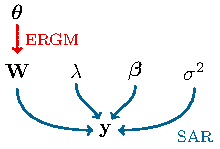
\includegraphics[scale=1]{figures-tikz/ergm.pdf}
		\caption{\acrshort{sar} with \acrshort{ergm} prior.}
		\label{fig:sar-ergm}
	\end{subfigure}
	\begin{subfigure}{0.45\textwidth}
		\centering
		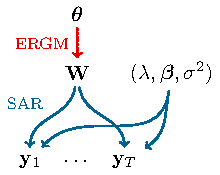
\includegraphics[scale=1]{figures-tikz/ergm-panel.pdf}
		\caption{\acrshort{sar} with \acrshort{ergm} prior (panel data).}
		\label{fig:sar-ergm-panel}
	\end{subfigure}
	\caption{\acrshort{dag} Representations.}
	\label{fig:dag-representation}
\end{figure}


\subsection{Priors: \gls{sar}}\label{sec:prior-sar}

We now specify the simplest case
where we assume that the parameter $\ttheta$ for the \gls{ergm} probability $\pr(\WW\given\ttheta)$ is known.
For each parameter in the \gls{sar} model, we specify the following priors:
\begin{align}\label{eq:prior}
	\begin{cases}
		\bbeta                &\sim    \Normal(\mmu_{\bbeta},\VV_{\bbeta}), \\
		\sigma^2              &\sim    \InverseGamma(a_{\sigma^2},b_{\sigma^2}), \\
		\lambda               &\sim    \Uniform(-1,1), \\
		\pr(\WW\given\ttheta) &\propto \exp(\ss(\WW)\T\ttheta).
	\end{cases}
\end{align}
The specification of $\bbeta$ and $\sigma^2$ are standard conjugate priors;
uniform prior for $\lambda$ is standard in Bayesian estimations of the \gls{sar} model
with known networks \parencite{lesage-pace-2009};
of course, we specify $\WW$ to follow \gls{ergm}.
This set of priors are represented in a \gls{dag} in \autoref{fig:sar-ergm}.
This setup, apart from the prior $\pr(\WW\given\ttheta)$ for the unknown network,
is standard in \gls{sar} literature where Bayesian methods are employed.

\subsection{Priors: \gls{ergm}}\label{sec:prior-ergm}

In practice, the researcher would not know \emph{a priori} the value of $\ttheta$.
Thus, we need to also specify a prior on the \gls{ergm} parameters.
The standard choice would be Gaussian priors,
same as the specifications in \cite{caimo-friel-2011}:
$\ttheta \sim \Normal(\mmu_{\ttheta},\VV_{\ttheta}).$

% The posterior of $\ttheta$ can not be sampled using standard \gls{mh}
% algorithm since the normalizing constant $z(\ttheta)$ is unknown. Fortunately,
% as mentioned in \autoref{sec:ergm-prior}, \cite{caimo-friel-2011} provided
% variants of the \gls{ex} algorithm for sampling this type of posterior
% efficiently.

\subsection{Panel Data}

In practice,
a single observation of $\yy$ and $\XX_{1},\XX_{2}$'s without observing $\WW$
contains too little information about $\WW$ to be useful.
\footnote{
	Clearly, with only one observation, the parameters of interest are not identified in the frequentist sense.
	As mentioned in \autoref{sec:introduction},
	\cite{de_paula-2023} provided a frequentist identification result
	of time-invariant unknown network in \gls{sar} with panel data.
	In a pure Bayesian sense,
	there is no problem of identification,
	i.e., identification is only a problem with the likelihood function.
	As long as a posterior distribution is defined,
	one can make valid Bayesian inference.
}
Thus, we introduce a time subscript $t=1,...,T$, i.e., we repeatedly observe realizations of $\yy_{t}$.
Explicitly, we now have a subscripted version of \eqref{eq:likelihood} as
\begin{align*}
	f(\yy_{t}\given\lambda,\WW,\bbeta,\sigma^2)
	&=
	(2\pi)^{-N/2}
	(\sigma^2)^{-N/2}
	\det(\MM)
	\exp \left( -\frac1{2\sigma^2} \norm{\MM\yy_{t}-\HH_{t}\bbeta} \right).
\end{align*}
And the likelihood of observing the entire data is
\begin{align*}
	f(\{\yy_{t}\}\given\lambda,\WW,\bbeta,\sigma^2)
	= \prod_{t} f_t(\yy_{t}\given\lambda,\WW,\bbeta,\sigma^2)
\end{align*}
where the subscripted $f_t$ simply denotes the dependency of $\XX_t$.
The \gls{dag} representation is shown in \autoref{fig:sar-ergm-panel}.
The conditional posteriors are presented in \autoref{app:derivation-of-posteriors}.
In subsequent discussions, we will focus on this case of having panel data.

\section{Sampling Procedure}\label{sec:sampling-procedure}

To estimate our model, we employ the Gibbs sampling algorithm.
In the following subsection, we describe the sampling strategy for each parameter.

\begin{algorithm}[t]
	\centering
	../paper/algorithmic-gibbs.tex
	\caption{Gibbs Sampling.}
	\label{alg:gibbs}
\end{algorithm}


\subsection{Sample Posterior \texorpdfstring{$\bbeta$}{beta} and \texorpdfstring{$\sigma^2$}{sigma-squared}}

For $\bbeta$ and $\sigma^2$,
standard normal-normal and normal-inverse-gamma conjugacy results apply immediately.
Their corresponding full conditional posterior densities are presented in
\autoref{app:posterior-beta} and \autoref{app:posterior-sigma-2} respectively.

\subsection{Sample Posterior \texorpdfstring{$\lambda$}{lambda}}

The posterior of $\lambda$ with a uniform prior assumes no known form, as shown in \autoref{app:posterior-lambda}.
Hence, \gls{mcmc} techniques must be utilized.
In \cite{lesage-pace-2009} and also \cite{ritter-tanner-1992},
their recommended the usage of \gls{gg} instead of \gls{mh} for efficiency.
However, in our case, we found that the efficiency gain in using \gls{gg} is not significant.
Furthermore, \gls{gg} tends to be more unstable compared to \gls{mh},
especially in the early phase of Gibbs sampling due to the unstableness of the likelihood function.
Therefore, a simple \gls{mh} algorithm is adopted for sampling posterior $\lambda$ in our case.

\subsection{Sample Posterior \texorpdfstring{$\WW$}{W}}

Technically, the posterior of $\WW$ also follows \gls{ergm}.
However, its form is not standard, which inhibits us to use standard packages such as \Verb"ergm"  in R.
Thus, a custom sampler utilizing a discrete variation of \gls{hmc} from \cite{pakman-paninski-2015} is adopted.
More implementation details can be found in \autoref{app:hmc}.

\subsection{Sample Posterior \texorpdfstring{$\ttheta$}{theta}}

The method for sampling posterior $\ttheta$,
the \gls{ex} algorithm, is directly adopted from \cite{caimo-friel-2011}.
As mentioned in \autoref{sec:ergm-prior}, sampling posterior $\ttheta$ is a \emph{double intractable} problem,
since the posterior density of $\ttheta$ is
\begin{align*}
	\pr(\ttheta\given\yy,\lambda,\WW,\bbeta,\sigma^2)
	&\propto \pr(\WW\given\ttheta)\pr(\ttheta)
	= \frac{1}{z(\ttheta)} \exp(\ttheta\T\ss(\WW)) \pr(\ttheta)
\end{align*}
where $z(\ttheta)$ is unknown to the researcher.
The \gls{ex} algorithm solves this problem by introducing an auxiliary state $\tilde\WW$,
which is sampled from \gls{ergm} with parameter $\ttheta$.
This auxiliary state is used to approximate the unknown normalizing constant $z(\ttheta)$.
\cite{caimo-friel-2011} further proposed the \gls{ads},
an extension of \gls{ex}, for better acceptance rate.
In our case,
we found that the additional complexity of the \gls{ads} is not worth the marginally better acceptance rate.
Thus, a basic \gls{ex} algorithm is implemented.

\dinkus

The full algorithm for posterior sampling is presented in \autoref{alg:gibbs}.
One detail to note is the order in which each parameter is sampled,
as different ordering will effect the convergence rate of the algorithm.
It is preferable that one first samples from $\bbeta$,
as a good starting $\bbeta$ quickly in the moves the likelihood in correct direction.
A bad choice would be to start with $\lambda$ or $\WW$,
since bad choices of either of these would greatly effect the matrix $(\II-\lambda\bar\WW)\inv$,
making the likelihood unstable.
Nevertheless, Gibbs sampling guarantees the convergence of the posterior samples,
regardless of ordering.
Further implementation details can be found at \autoref{app:implementation-details}.

\section{Simulation Study}\label{sec:simulation-study}

In this section,
we present three simulation studies.
The first study uses a artificial network generated directly from an \gls{ergm};
the second study uses the \emph{Sampson's Monk} network (directed) with artificially generated data;
the their study uses the \emph{Zachary's Karate Club} network (undirected) also with artificially generated data.

\subsection{Basic \gls{ergm}}\label{subsec:P}

\begin{figure}[t]
	\centering
	\begin{subfigure}{0.31\textwidth}
		\centering
		\includegraphics[width=0.9\textwidth]{figures/panel.pdf}
		\caption{Network}
	\end{subfigure}
	\begin{subfigure}{0.31\textwidth}
		\centering
		\includegraphics[width=\textwidth]{figures/P1-true-W.pdf}
		\caption{Adjacency Matrix}
	\end{subfigure}
	\caption{Simulated \acrshort{ergm} network for \autoref{subsec:P}.}
	\label{fig:P}
	\caption*{\footnotesize\emph{Note}: The white dots in the adjacency matrix denotes mutuality.}
\end{figure}

\begin{figure}[t]
	\centering
	\begin{subfigure}{0.31\textwidth}
		\centering
		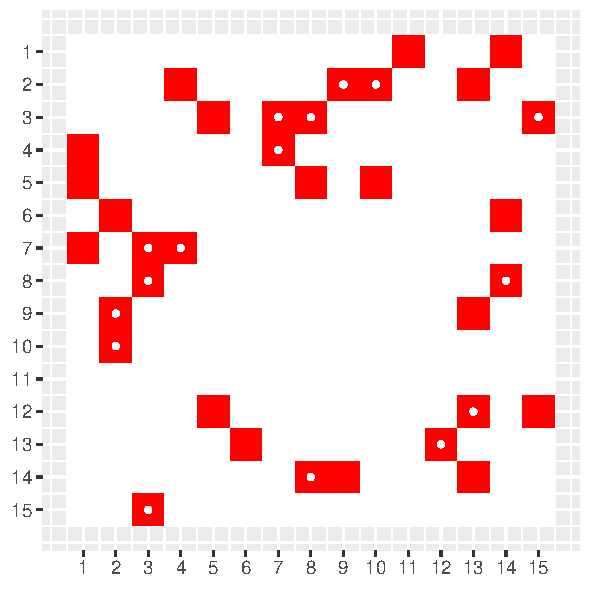
\includegraphics[width=\textwidth]{figures/penta-W.pdf}
		\caption{True Adjacency Matrix}
	\end{subfigure}
	\begin{subfigure}{0.31\textwidth}
		\centering
		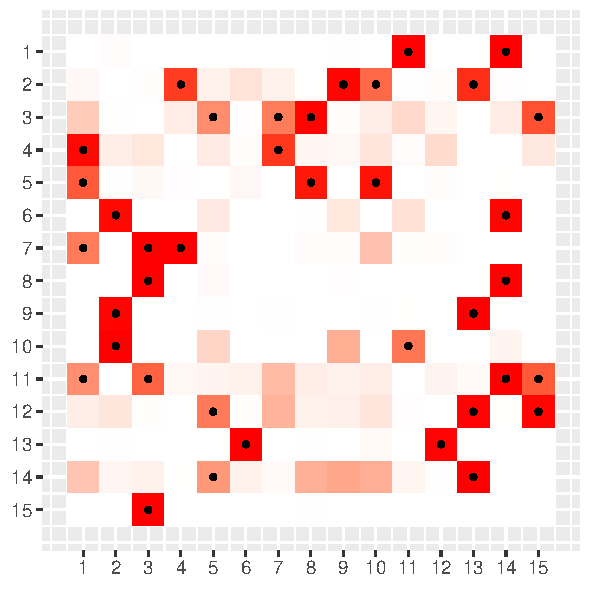
\includegraphics[width=\textwidth]{figures/P10-posterior-W.pdf}
		\caption{P10}
	\end{subfigure}
	\begin{subfigure}{0.31\textwidth}
		\centering
		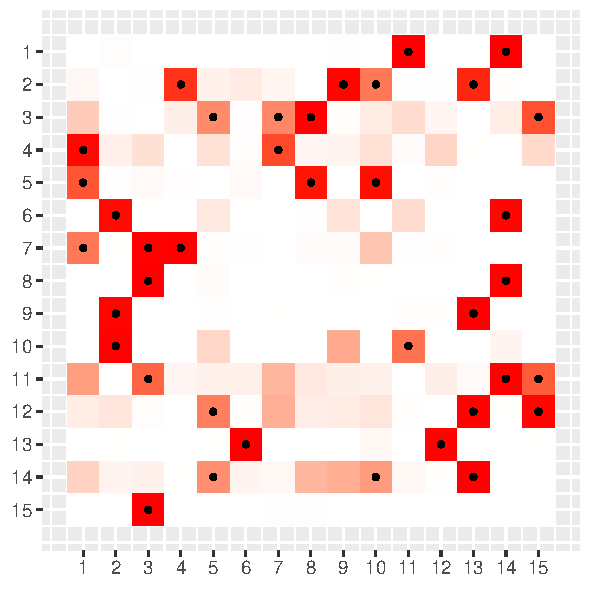
\includegraphics[width=\textwidth]{figures/P11-posterior-W.pdf}
		\caption{P11}
	\end{subfigure}
	\begin{subfigure}{0.31\textwidth}
		\centering
		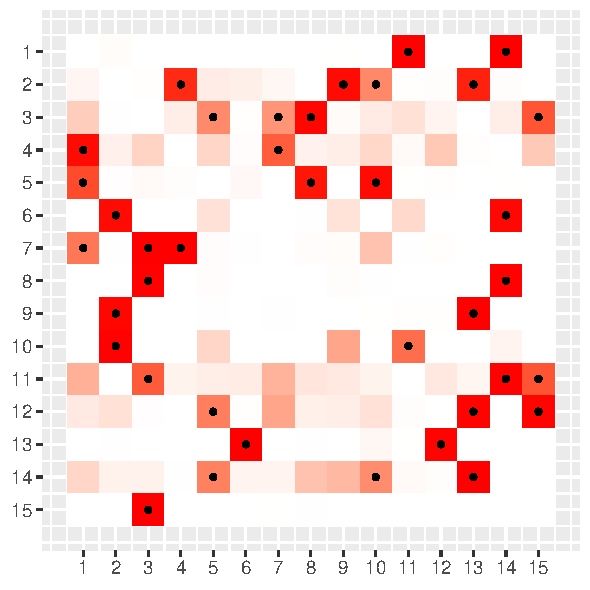
\includegraphics[width=\textwidth]{figures/P12-posterior-W.pdf}
		\caption{P12}
	\end{subfigure}
	\begin{subfigure}{0.31\textwidth}
		\centering
		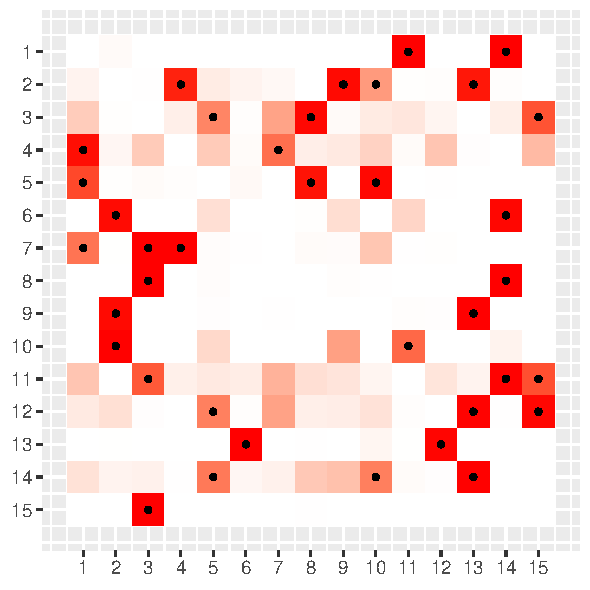
\includegraphics[width=\textwidth]{figures/P13-posterior-W.pdf}
		\caption{P13}
	\end{subfigure}
	\begin{subfigure}{0.31\textwidth}
		\centering
		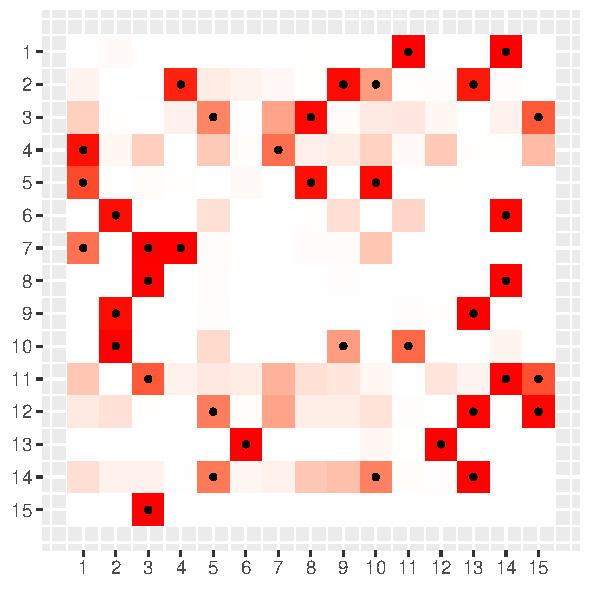
\includegraphics[width=\textwidth]{figures/P14-posterior-W.pdf}
		\caption{P14}
	\end{subfigure}
	\caption{Posterior Adjacency Matrices.}
	\label{fig:P1}
	\caption*{\footnotesize\emph{Note}: The black dots in the posterior adjacency matrices denotes the probability of entry being one exceeding $50\%$.}
\end{figure}

\begin{figure}[t]
	\centering
	\begin{subfigure}{0.31\textwidth}
		\centering
		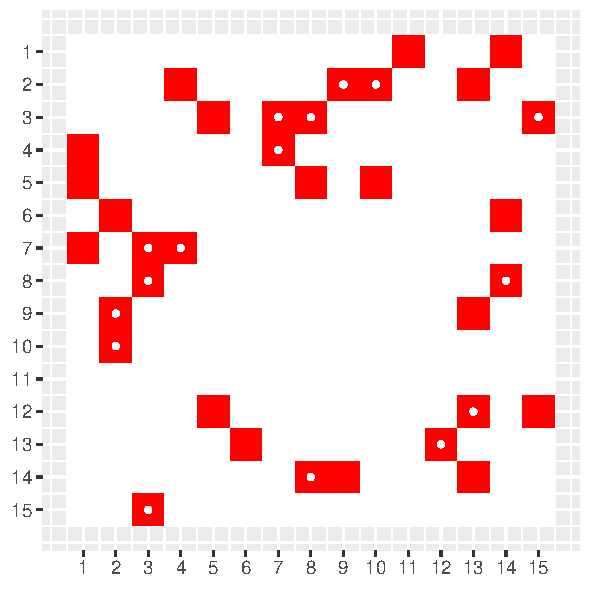
\includegraphics[width=\textwidth]{figures/penta-W.pdf}
		\caption{True Adjacency Matrix}
	\end{subfigure}
	\begin{subfigure}{0.31\textwidth}
		\centering
		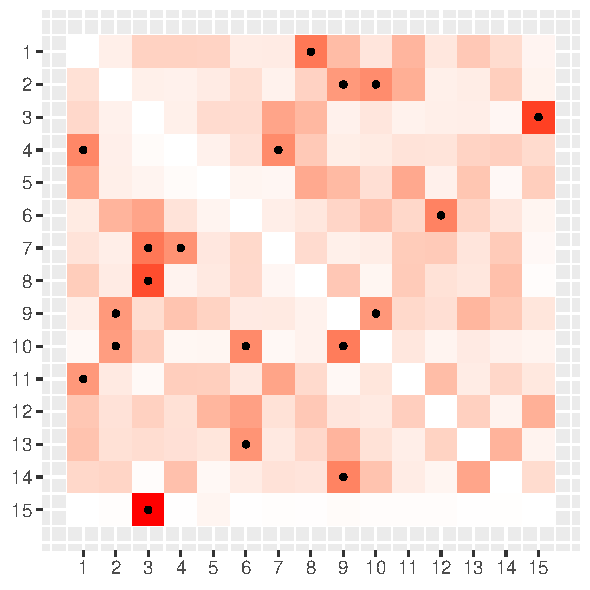
\includegraphics[width=\textwidth]{figures/P20-posterior-W.pdf}
		\caption{P20}
	\end{subfigure}
	\begin{subfigure}{0.31\textwidth}
		\centering
		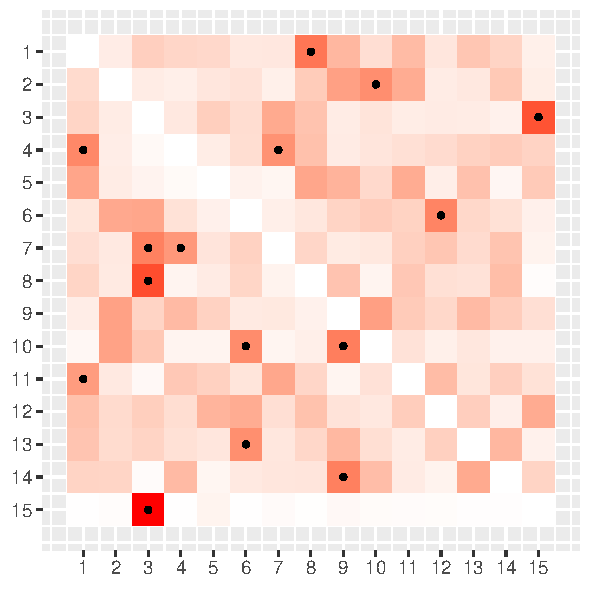
\includegraphics[width=\textwidth]{figures/P21-posterior-W.pdf}
		\caption{P21}
	\end{subfigure}
	\begin{subfigure}{0.31\textwidth}
		\centering
		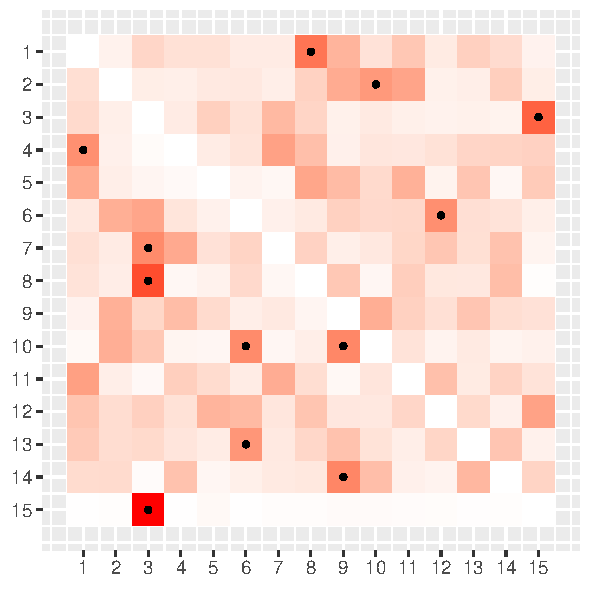
\includegraphics[width=\textwidth]{figures/P22-posterior-W.pdf}
		\caption{P22}
	\end{subfigure}
	\begin{subfigure}{0.31\textwidth}
		\centering
		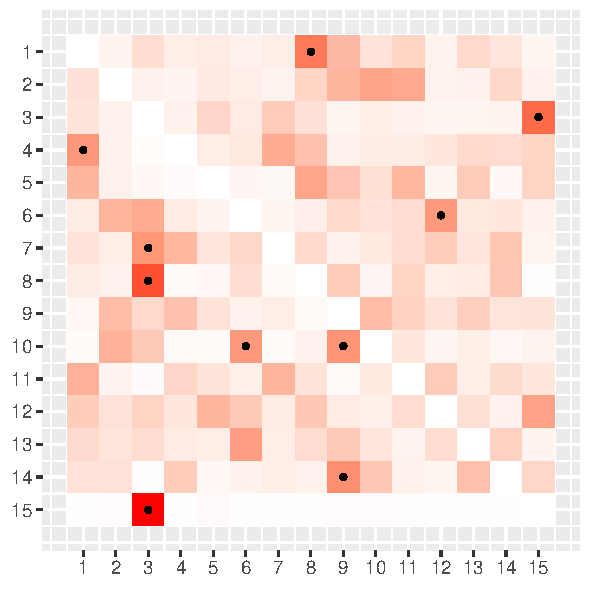
\includegraphics[width=\textwidth]{figures/P23-posterior-W.pdf}
		\caption{P23}
	\end{subfigure}
	\begin{subfigure}{0.31\textwidth}
		\centering
		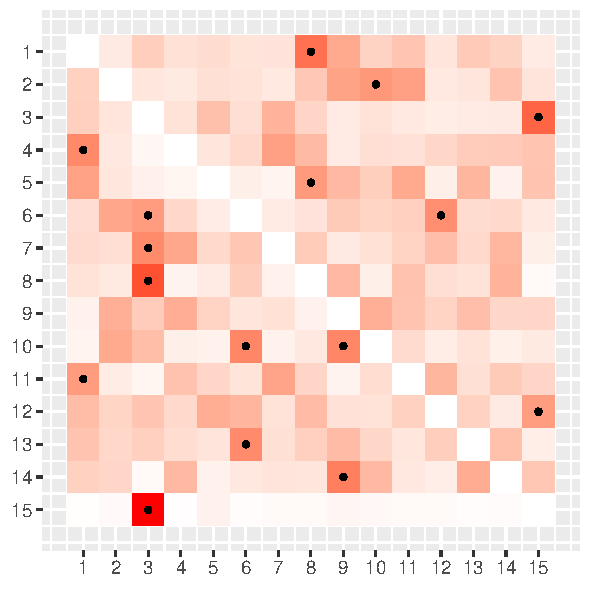
\includegraphics[width=\textwidth]{figures/P24-posterior-W.pdf}
		\caption{P24}
	\end{subfigure}
	\caption{Posterior Adjacency Matrices.}
	\label{fig:P2}
\end{figure}


In this first simulation study,
we consider a data set that contains $N=15$ nodes and a panel length of $T=12$.
\footnote{
	Note that with an entirely unknown network,
	it is impossible to recover $\WW$ with \gls{mle} given this panel length.
	Hence, we do not intend to compare the efficiency of our results with \gls{mle} or frequentist methods.
}
The network, shown in \autoref{fig:P},
is generated from an \gls{ergm}
with sufficient statistics $\text{\Verb"edges"}=-2$ and $\text{\Verb"mutual"}=2$.
Two groups of simulations are run here:
\begin{itemize}[leftmargin=\widthof{Group P1: }]
	\item[\itemlabel{group:P1}{Group P1}:]
		$\XX_1$ is an $N\times 1$ matrix of exogenous variables generated from a normal distribution and $\XX_{2}$ equals $\XX_{1}$.
	\item[\itemlabel{group:P2}{Group P2}:]
		$\XX_1$ is an $N\times 2$ matrix of exogenous variables generated from a normal distribution.
\end{itemize}
That is, \ref{group:P1} is run \emph{with} correlated effect while \ref{group:P2} \emph{without}.
The main focus of this first simulation study is on different prior specifications of $\ttheta$ and model specification.
The simulations results of the parameters are reported in \autoref{tab:P1} respectively;
and the results of the adjacency matrices are shown in \autoref{fig:P1} and \autoref{fig:P2} respectively.
The results are obtained by running \autoref{alg:gibbs} for $3000$ iterations and discarding the first $10\%$ of iterations as burn-in.

\paragraph{Posterior Inference on $\lambda$.}

In all specifications presented in \autoref{tab:P1},
no significant result is obtained for $\lambda$.
This is true even for larger specification of $\lambda$ (for $\lambda=0.15$ and $\lambda=0.2$).
\footnote{
	The simulation results of $\lambda=0.15$ and $\lambda=0.2$ is not presented here,
	since the results are almost identical to \autoref{tab:P1},
	except for the posterior mean of $\sigma^2$.
	The posterior mean of $\sigma^2$ with larger $\lambda$ is larger than those presented in \autoref{tab:P1},
	since the unstable nature of $(\II-\lambda\bar\WW)\inv$ is reflected mostly in $\sigma^2$.
}
In an \gls{sar} model (with Bayesian treatment) where the network is known,
we essential make inference on the posterior distribution $\pr(\lambda,\bbeta,\sigma^2\given\{\yy_{t}\},\WW)$;
however, in our case, our inference is on the distribution $\pr(\lambda,\WW,\bbeta,\sigma^2\given\{\yy_{t}\})$.
Whether or not $\WW$ is conditioned changes the distribution of $\lambda$ substantially.

One the other hand,
as presented in the lower half of \autoref{tab:P1}
we obtain all significant results for $\lambda$.
This is clearly related to the \gls{dgp}.
However, the exact nature of why this is unclear to the author.

\paragraph{Posterior Inference on $\WW$.}

In \autoref{fig:P1},
a gradient between white and red is used to represent the posterior mean:
the darker the color, the closer if the mean to $1$;
similarly, the lighter, the closer is the mean to $0$.

Overall, the retrieval of matrix $\WW$ is surprisingly good in all specifications with only $T=12$.
As expected,
the posterior mean is noisier if the prior belief is less defined.
Nevertheless, in all specifications,
most entries are completely white, i.e.,
the information from the likelihood function
is sufficiently strong to rule out many improbable links.
\footnote{
	In many applications,
	It might be necessary to obtain a binary adjacency matrix from the posterior samples,
	not just the posterior mean.
	From a purely decision theoretic point of view,
	we need to specify a specific loss function for this objective.
	One possible candidate is the zero-one loss,
	which corresponds to the \gls{map} decision rule.
	However, the loss function would depend on the application in different scenarios.
	Hence, we simply present the posterior mean of $\WW$ as a convenient summary of the posterior distribution.

	From a more practical perspective,
	one can simply categorise the posterior mean of $\WW$ by some threshold value
	and declare a certain link is retrieved if the posterior mean surpasses the value.
	In decision theoretic framework,
	we can obtain this decision rule by considering the following loss function
	\begin{align*}
		L(\hat\WW,\WW_0) = \#\{(i,j):\hat\WW_{i,j}\neq(\WW_{0})_{i,j}\},
	\end{align*}
	that is, counting the total miss-categorized entries.
	It is straightforward to derive that the decision rule corresponding to this loss function should be
	\begin{align*}
		\hat\WW_{i,j} = \one
		\left\{
		\pr((\WW_0)_{i,j}=1\given\{\yy_{t}\}) \geq 0.5
		\right\},
	\end{align*}
	that is, let the $(i,j)$-entry of the decision $\hat\WW$ be $1$ if the posterior probability the entry being one is over $0.5$.
	In the empirical illustration from \cite{krisztin-piribauer-2022},
	they adopted a similar strategy by categorizing the posterior mean of the adjacency matrix in three categories
	via cut-off values $0.5$ and $0.75$.
}

Compared to the results shown in \autoref{fig:P1},
it is clear that the posteriors in \autoref{fig:P2} are a lot less defined.
A heuristic explanation is that the term $\bar\WW\XX_2\bbeta_2$ provides a lot of information about $\WW$,
where as a lack of such term makes the exact entries of $\WW$ more ambiguous.
%This might be due to the fact that there are no $\XX_2$'s included in the second group,
%which led to less information about $\WW$ from the data.

\paragraph{Posterior Inference on $\ttheta$.}

Different prior distributions of $\ttheta$ leads to different result:
the more specific and ``correct'' the prior is, the less noisy posterior mean of $\WW$ is.
\footnote{
	In this case,
	there is a ``correct'' prior since the network is generated from a known \gls{ergm} with known parameters.
	Of course, there is no ``correct'' prior in the Bayesian framework.
	Hence, by ``correct'' we simply mean closer to the \gls{ergm} that generates this specific network.
}
The most important difference is whether each $\ttheta$ obtains significant results.
In all cases, $\ttheta_{\text{\Verb"edges"}}$ is significant ($95\%$ credible interval),
since \emph{sparseness} is perhaps the most important aspect of this simulated matrix;
on the other hand,
$\ttheta_{\text{\Verb"mutual"}}$ obtains significant result
only in the case where the prior belief on it is very strong (first case in \autoref{tab:P1}).
Nevertheless, all prior specifications leads to roughly similar posterior inferences.
This result is similar to the results reported in \cite{krisztin-piribauer-2022},
as they also reported that the ``sparsity'' parameter can be effectively chosen by the model,
rather than specifying it \emph{a priori}.
%Inference about $\ttheta$ is perhaps more of interest than inference about $\WW$.

\dinkus

The results of this simulation is promising.
However, as one can see in \autoref{fig:P},
this simulated networks is not what we typically would observe in application.
In the next two sections, we perform simulation on two well-known networks.

\subsection{Sampson's Monk: Directed Network}\label{subsec:S}

\begin{figure}[t]
	\centering
	\begin{subfigure}{0.31\textwidth}
		\centering
		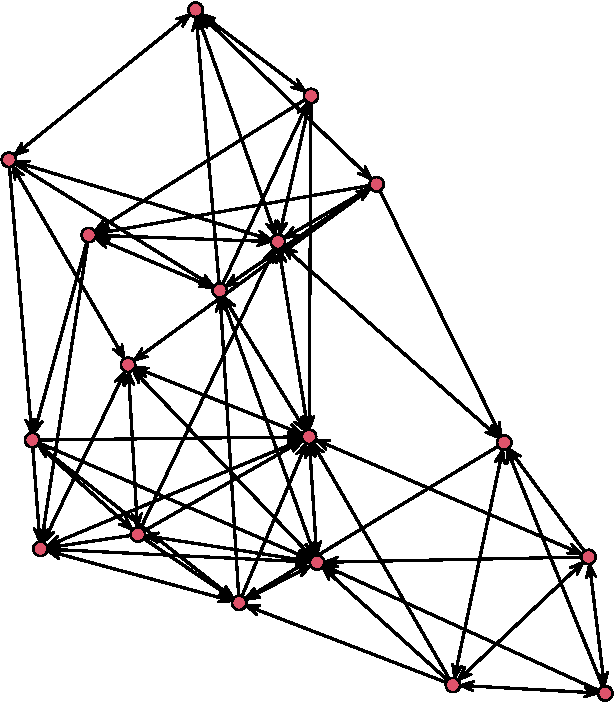
\includegraphics[height=\textwidth]{figures/sampson.pdf}
		\caption{Network}
	\end{subfigure}
	\begin{subfigure}{0.31\textwidth}
		\centering
		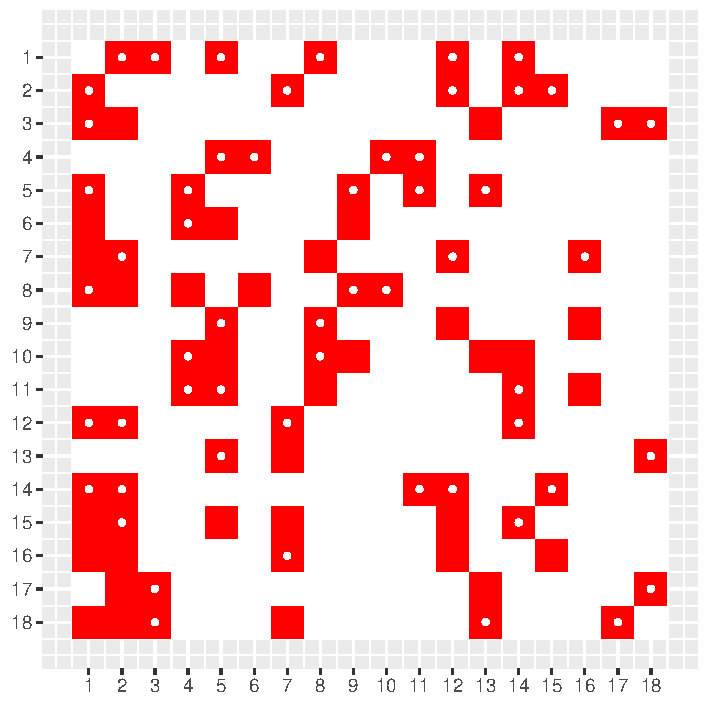
\includegraphics[width=\textwidth]{figures/sampson-W.pdf}
		\caption{Adjacency matrix}
	\end{subfigure}
	\caption{Sampson's Monk}
	\label{fig:S}
\end{figure}

\begin{figure}[h]
	\centering
	\begin{subfigure}{0.31\textwidth}
		\centering
		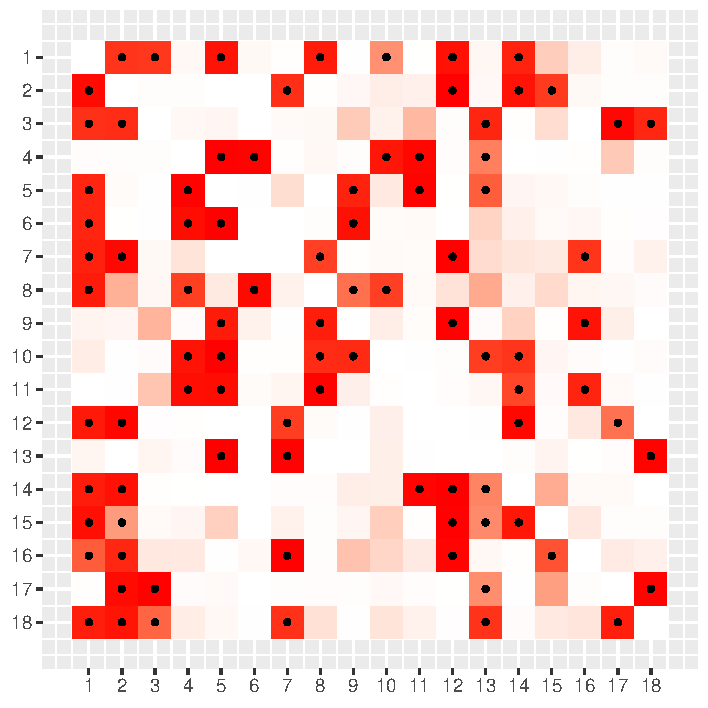
\includegraphics[width=\textwidth]{figures/S10-posterior-W.pdf}
		\caption{S10 ($T$: 18)}
	\end{subfigure}
	\begin{subfigure}{0.31\textwidth}
		\centering
		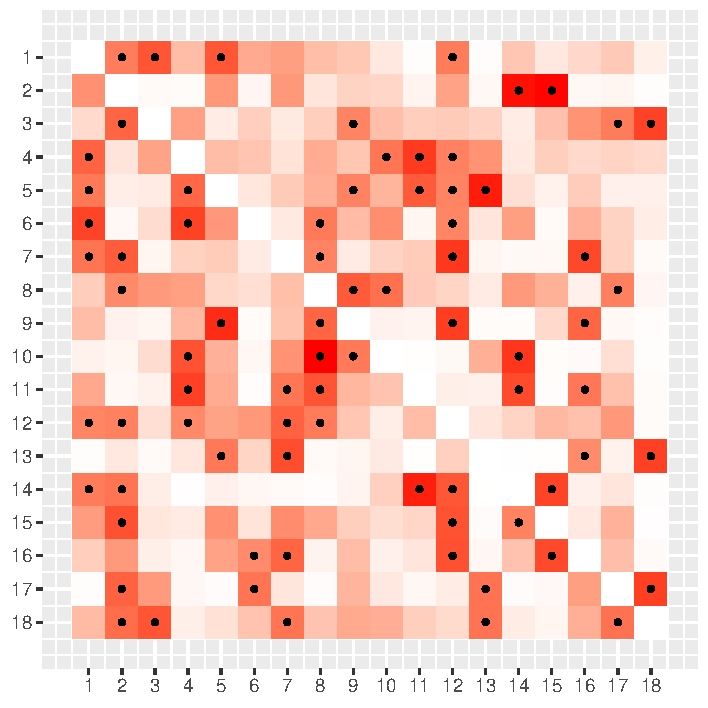
\includegraphics[width=\textwidth]{figures/S11-posterior-W.pdf}
		\caption{S11 ($T$: 12)}
	\end{subfigure}
	\begin{subfigure}{0.31\textwidth}
		\centering
		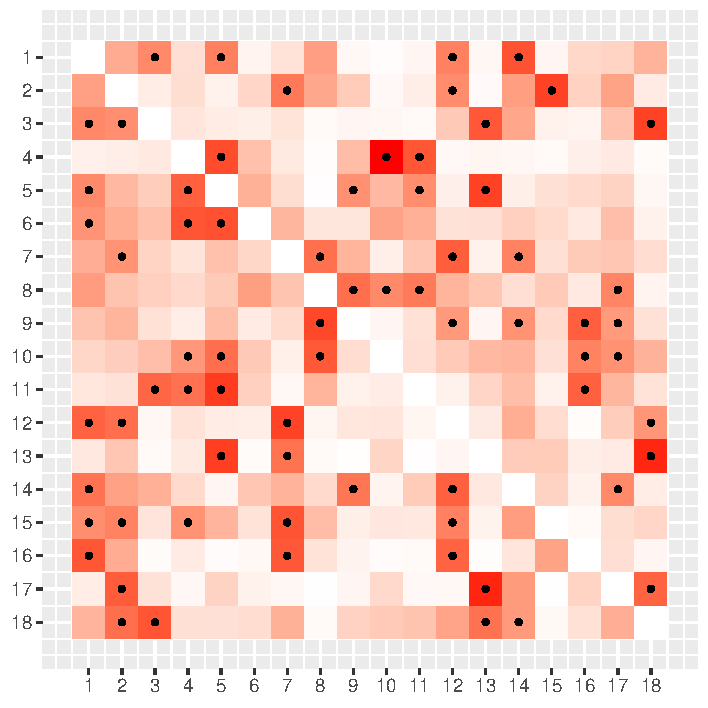
\includegraphics[width=\textwidth]{figures/S12-posterior-W.pdf}
		\caption{S12 ($T$: 8)}
	\end{subfigure}
	\begin{subfigure}{0.31\textwidth}
		\centering
		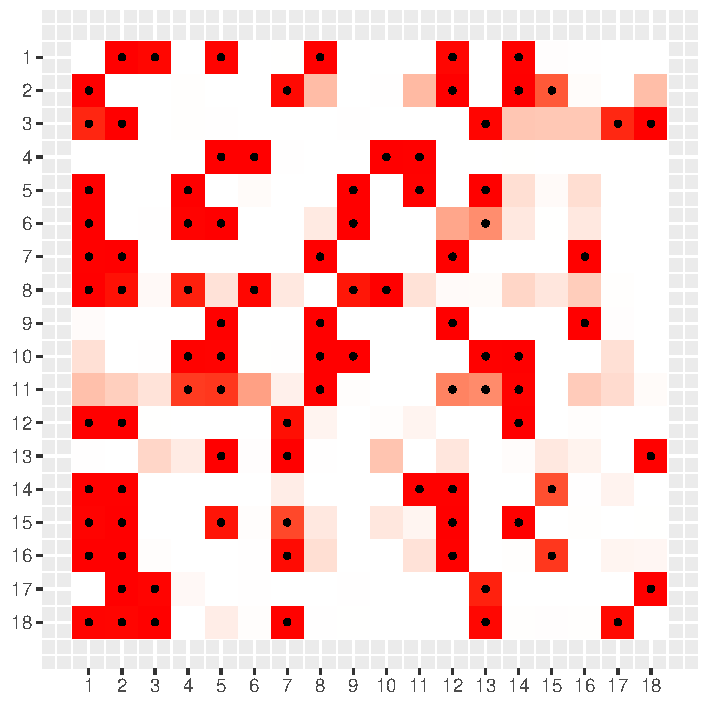
\includegraphics[width=\textwidth]{figures/S20-posterior-W.pdf}
		\caption{S20 ($T$: 18)}
	\end{subfigure}
	\begin{subfigure}{0.31\textwidth}
		\centering
		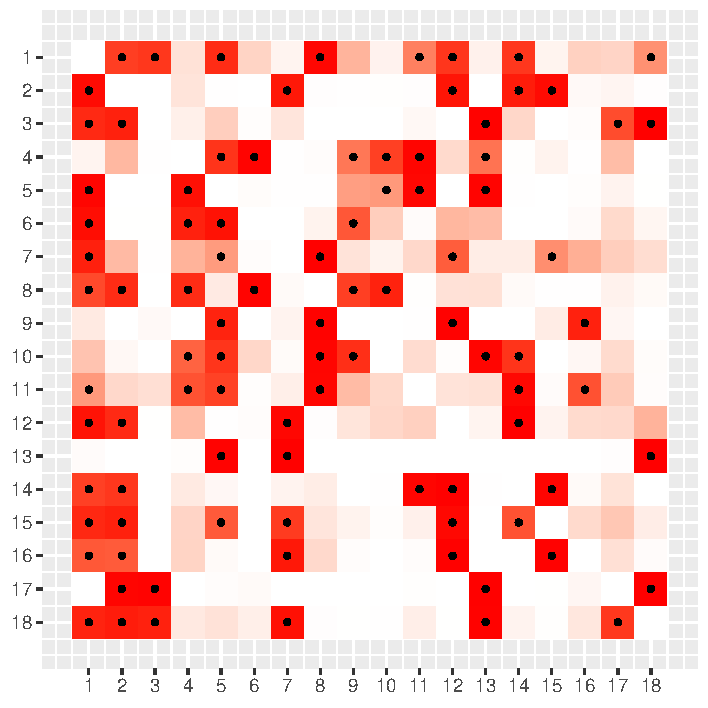
\includegraphics[width=\textwidth]{figures/S21-posterior-W.pdf}
		\caption{S21 ($T$: 12)}
	\end{subfigure}
	\begin{subfigure}{0.31\textwidth}
		\centering
		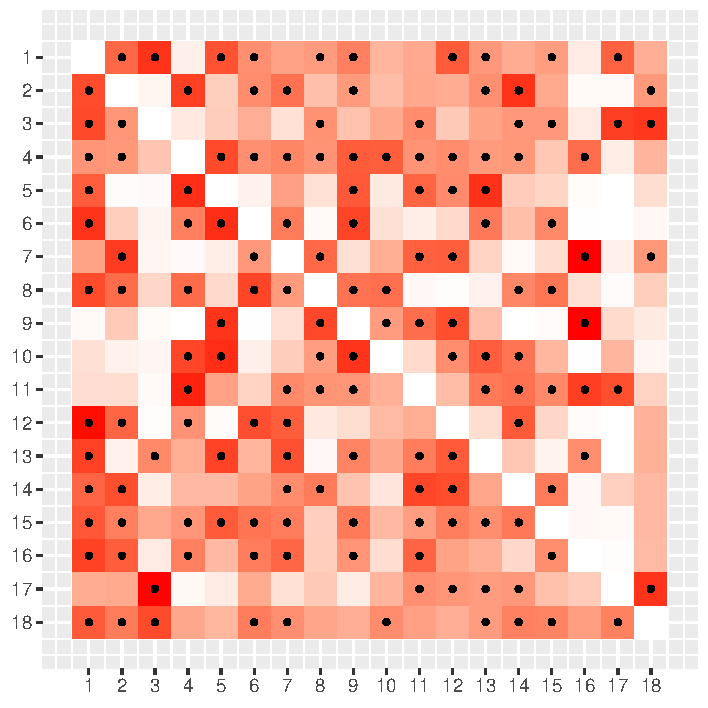
\includegraphics[width=\textwidth]{figures/S22-posterior-W.pdf}
		\caption{S22 ($T$: 8)}
		\label{fig:S22}
	\end{subfigure}
	\caption{Posterior Adjacency Matrices.}
	\label{fig:S1}
\end{figure}


In this simulation, we consider Sampson's monk network ($N=18$), as shown in \autoref{fig:S}.
A characteristic of the Sampson's monk network is that it is a lot less sparse compared to the network used in \autoref{subsec:P}.
This fact will be reflected in the simulation we see later.
Similar to the setting in \autoref{subsec:P},
we investigate two groups of simulations:
\begin{enumerate}[leftmargin=\widthof{Group S1: }]
	\item[\itemlabel{group:S1}{Group S1}:]
		$\XX_1$ is an $N\times 2$ matrix of exogenous variables
		with the first column generated from a normal distribution and the second column generated from a Bernoulli distribution.
		The second column is held constant across time to simulate characteristics that is time-invariant.
		Also, in this group $\XX_{2}$ is set to equal to $\XX_{1}$.
		The coefficients corresponding to the exogenous effects are larger than the coefficients corresponding to the correlated effects.
	\item[\itemlabel{group:S2}{Group S2}:]
		Similarly,
		$\XX_1$ and $\XX_2$ are $N\times 2$ matrices of exogenous variables
		with the first column generated from a normal distribution
		and the second column generated from a Bernoulli distribution that is held constant across time.
		But in this group,
		some correlated effects are larger than some exogenous effects.
\end{enumerate}
Three \gls{ergm} terms
(\Verb"edges", \Verb"mutual", and \Verb"ctriad") are incorporated in the estimation.
The goal of this simulation group is to see how the relative size of the correlated and exogenous effects affect the estimation quality.
We also vary the panel length observed by the econometrician in the simulations.

The results of \ref{group:S1} and \ref{group:S2} are presented in \autoref{tab:S1} and \autoref{fig:S1}.
\footnote{
	The \emph{true} $\ttheta$ presented in \autoref{tab:S1} is, of course, not literally \emph{true}.
	It is the \gls{ergm} estimate of the parameters given the network.
}
The main finding is intuitive and easily observed in \autoref{fig:S1}:
the shorter the panel length,
the less defined the posterior distributions, especially in the posterior distribution of the adjacency matrix.
Also notice that the posterior mean of $\WW$ is somewhat less defined than the results obtained in \autoref{subsec:P},
this is perhaps due to the fact that the Sampson's monk network is more complex than the artificial network used in \autoref{subsec:P}.

Comparing \ref{group:S1} and \ref{group:S2},
it seems like \ref{group:S2} performs better in terms of adjacency matrix recovery with panel length $T=18$ and $T=10$.
However, in the simulation with panel length $T=8$,
it seems like the posterior network is nearly degenerate,
i.e., a plurality of the entries in the posterior adjacency matrix appear over $50\%$.
The problem of degeneracy is characterized by that
the sampled network adjacency matrix using \gls{mcmc} techniques converges to a matrix with all entries being one.
This problem is well-known in the literature of \gls{ergm}, see e.g., \cite{handcock-2003} and \cite{rinaldo-fienberg-zhou-2009}.
In certain specifications with the Sampson's monk network,
the sampling of posterior adjacency network tend to degenerate.
However, in many cases when degeneracy occurs, we can normalize the posterior mean of the adjacency matrix and obtain somewhat reasonable results.
This is perhaps due to the fact that this particular network is not very sparse and the panel length is too short,
but still some information about the network is retained.
%However, \autoref{fig:S22} is not entirely degenerate.
%One can still make out the outline of the true matrix in the posterior mean.

In terms of the other parameters,
similar to the results in \autoref{subsec:P},
we cannot obtain significant result for $\lambda$ in \ref{group:S1} consistently.
The exogenous and correlated effects $\bbeta$ are estimated reasonably well, except for smaller effect sizes.
This is a general problem across all econometric models,
not a insufficiency of our approach.
The estimations for $\sigma^2$ worsen when panel length is reduced,
which is also to be expected.

%The results of the second simulation group is presented in \autoref{tab:S-2} and \autoref{fig:S-posterior-2}.
%In this simulations, we vary the variance of the exogenous variable $\XX_{1}$.
%Similar to the previous simulation,
%we held $\XX_{2}$ to be constant across time.

%Comparing \ref{group:S1} and \ref{group:S2},

%The main finding is that the variance in $\XX$ (especially $\XX_1$) affects the posterior inference significantly.
%As show in \autoref{fig:K-posterior-2},
%as the variance of the exogenous variable $\XX_{1}$ decreases,
%the noise in posterior distribution increases considerably.
%This is also to be expected, since the only information we as the econometrician observes is $\{\yy_{t},\XX_{t}\}$.
%When the variance in $\XX$ is relatively small,
%the likelihood function entails little information about the entire model,
%especially the high-dimensional adjacency matrix.
%Nonetheless, this is a general problem across all econometric/statistical models,
%not a insufficiency of our approach.

\dinkus

Overall, we still obtain reasonable estimates for all specifications,
even if the panel length is smaller than $N$.

\subsection{Zachary's Karate Club: Undirected Network}\label{subsec:K}

\begin{figure}[t]
	\centering
	\begin{subfigure}{0.31\textwidth}
		\centering
		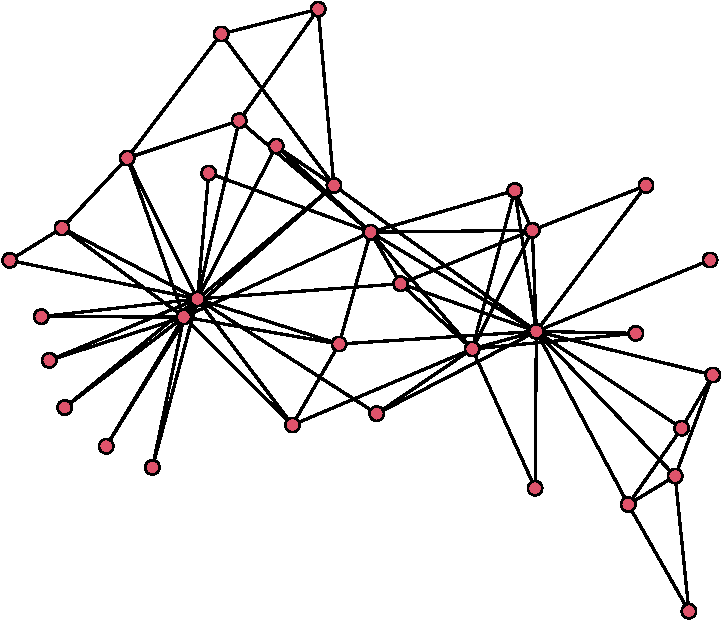
\includegraphics[width=\textwidth]{figures/zach.pdf}
		\caption{Network}
	\end{subfigure}
	\begin{subfigure}{0.31\textwidth}
		\centering
		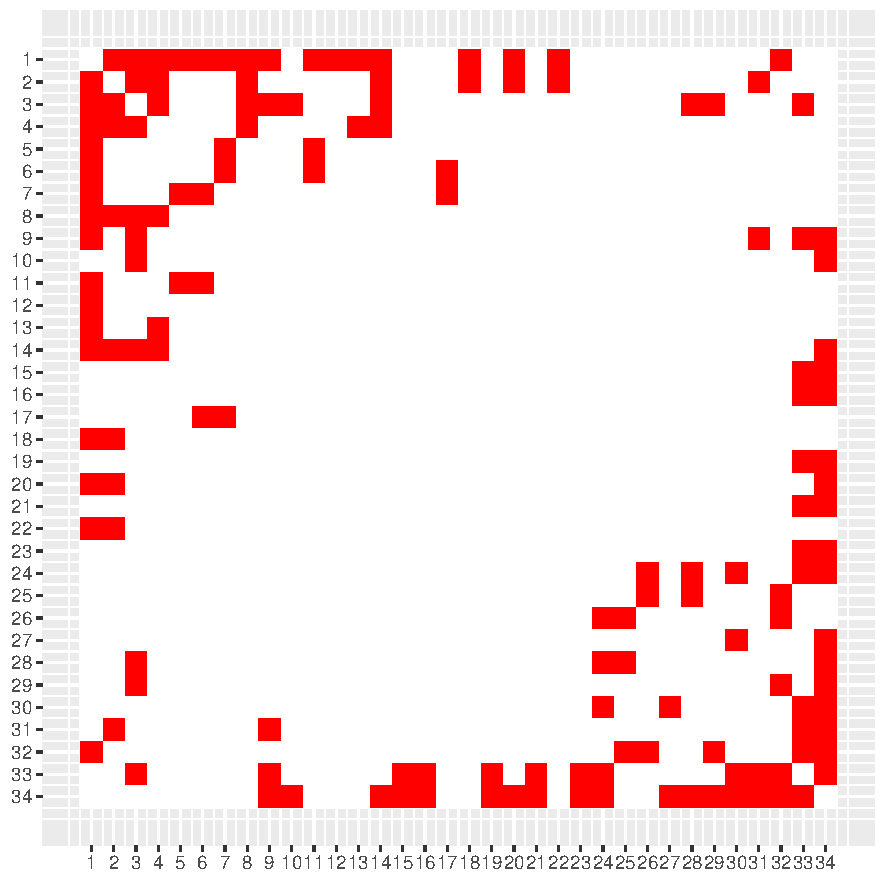
\includegraphics[width=\textwidth]{figures/zach-W.pdf}
		\caption{Adjacency Matrix}
	\end{subfigure}
	\caption{Zachary's Karate Club}
	\label{fig:K}
\end{figure}

\begin{figure}[h]
	\centering
	\begin{subfigure}{0.31\textwidth}
		\centering
		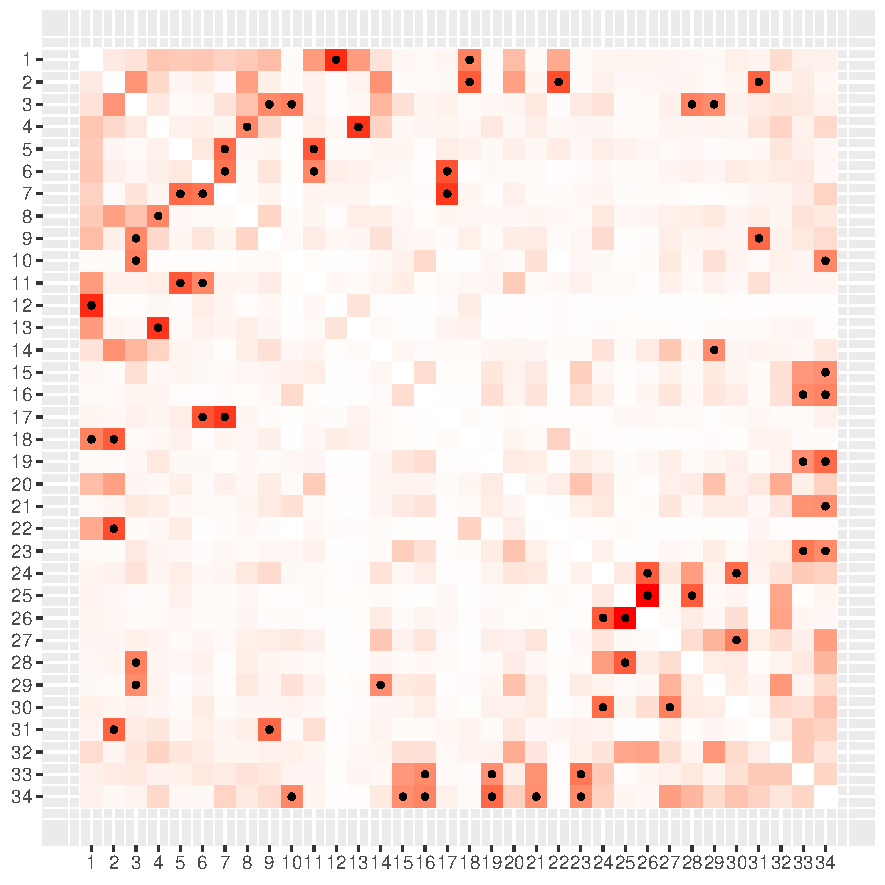
\includegraphics[width=\textwidth]{figures/K10-posterior-W.pdf}
		\caption{K10 ($T: 15$)}
	\end{subfigure}
	\begin{subfigure}{0.31\textwidth}
		\centering
		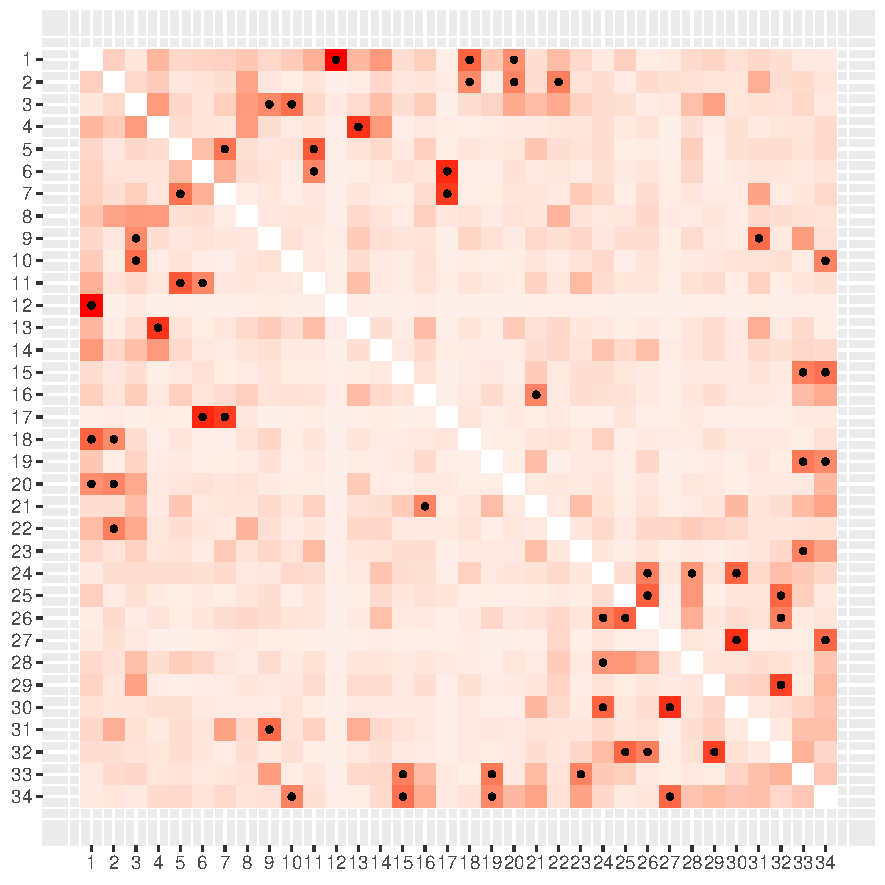
\includegraphics[width=\textwidth]{figures/K11-posterior-W.pdf}
		\caption{K11 ($T: 12$)}
	\end{subfigure}
	\begin{subfigure}{0.31\textwidth}
		\centering
		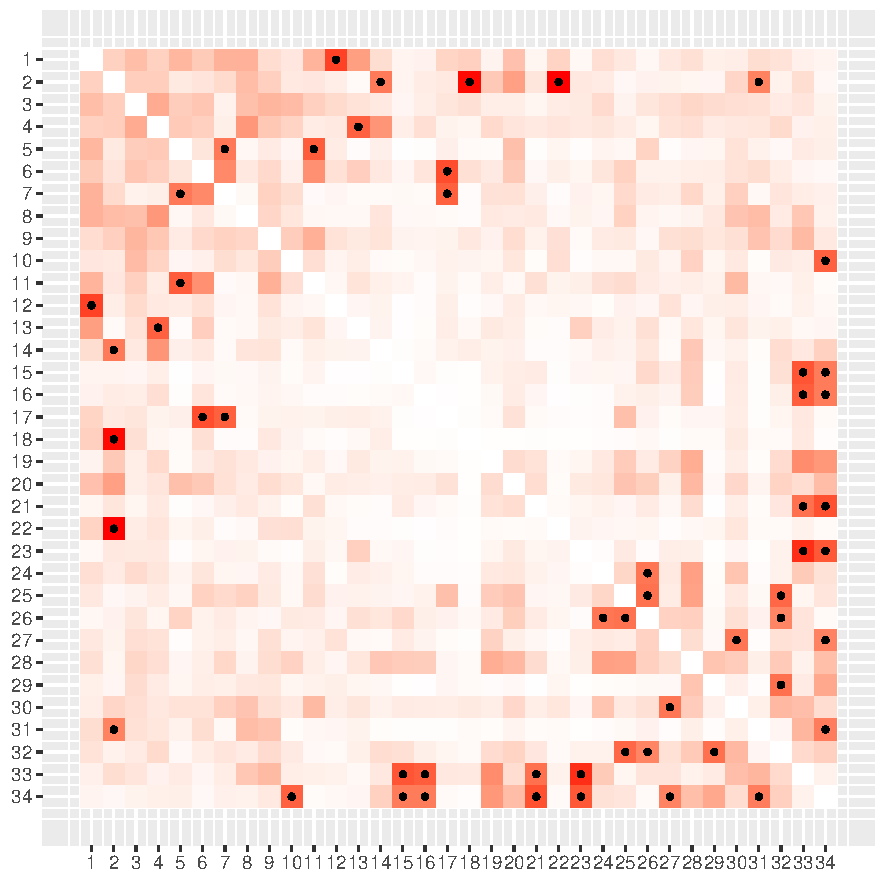
\includegraphics[width=\textwidth]{figures/K12-posterior-W.pdf}
		\caption{K12 ($T: 10$)}
	\end{subfigure}
	\begin{subfigure}{0.31\textwidth}
		\centering
		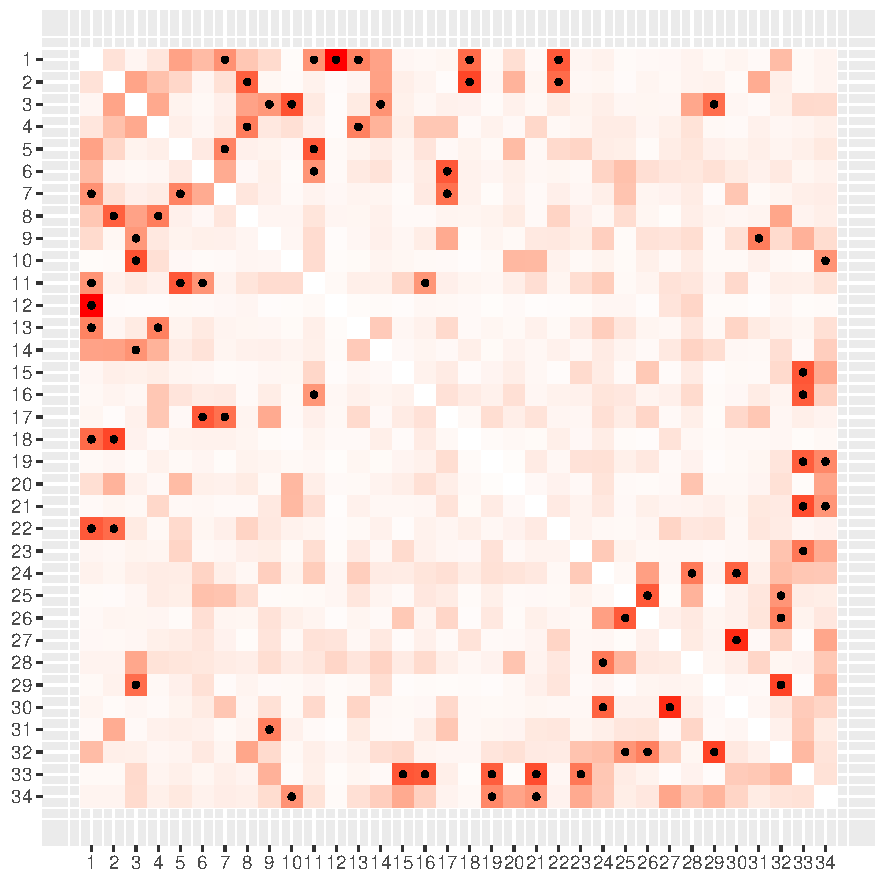
\includegraphics[width=\textwidth]{figures/K20-posterior-W.pdf}
		\caption{K20 ($T: 15$)}
	\end{subfigure}
	\begin{subfigure}{0.31\textwidth}
		\centering
		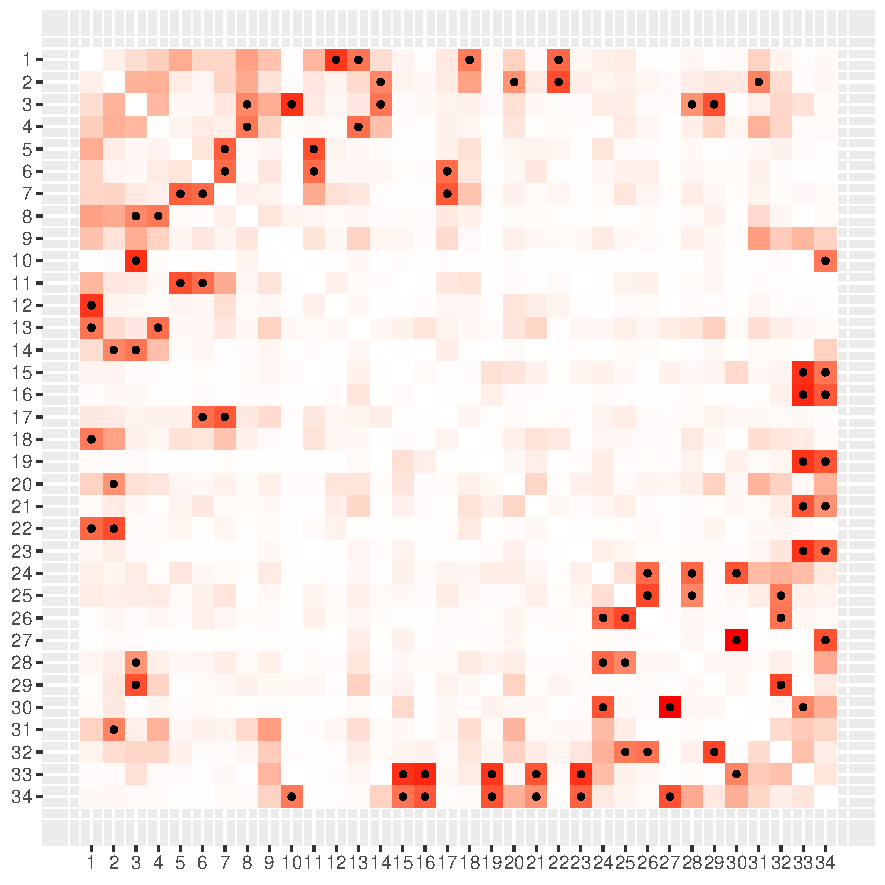
\includegraphics[width=\textwidth]{figures/K21-posterior-W.pdf}
		\caption{K21 ($T: 12$)}
	\end{subfigure}
	\begin{subfigure}{0.31\textwidth}
		\centering
		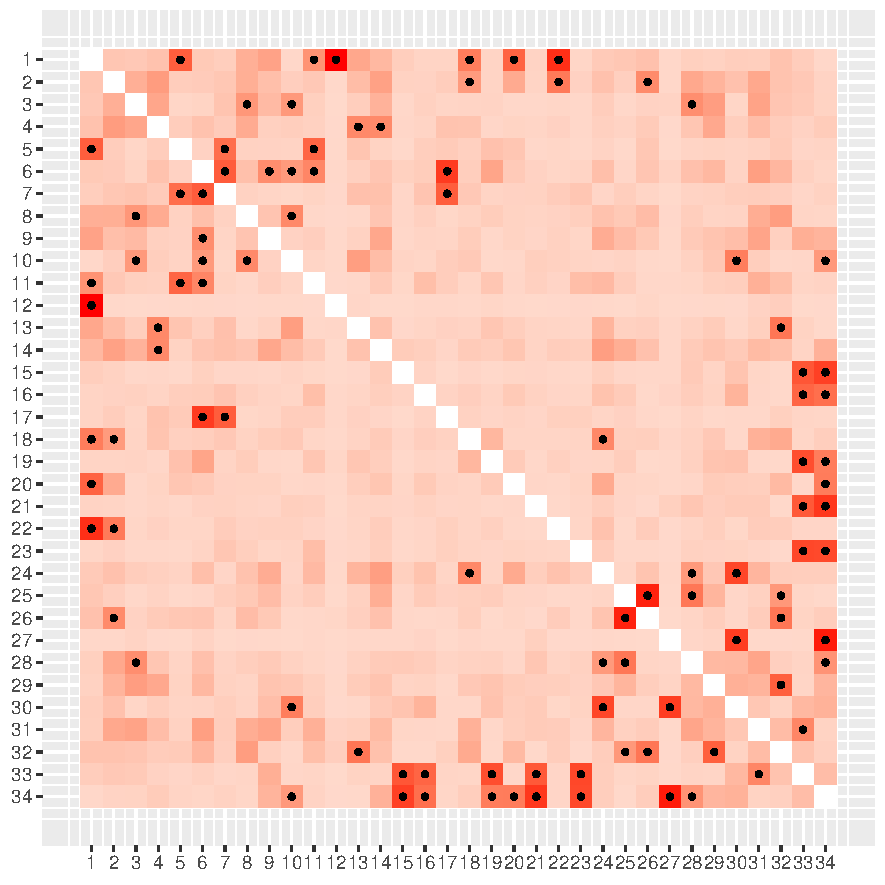
\includegraphics[width=\textwidth]{figures/K22-posterior-W.pdf}
		\caption{K22 ($T: 10$)}
	\end{subfigure}
	\caption{Posterior Adjacency Matrices.}
	\label{fig:K1}
\end{figure}


In this last simulation, we consider Zachary's karate club network ($N=34$), as shown in \autoref{fig:K}.
This network is considerably larger ($34\cdot(34-1)/2=561$ free elements in the adjacency matrix)
than the previous cases.
Furthermore, a symmetric adjacency matrix poses extra problems when it comes to sampling procedure,
since specialised functions that calculates the likelihood ratio efficiently are needed.

One simulation group is presented here:
\begin{itemize}[leftmargin=\widthof{Group K1: }]
	\item[\itemlabel{group:K1}{Group K1}:]
		$\XX_1$ is an $N\times 2$ matrix of exogenous variables.
		The first column is generated from a normal distribution,
		the second column is generated from a Bernoulli distribution.
		$\XX_2$ is an $N\times 1$ matrix identical to the first column of $\XX_1$.
		The endogenous effect of this group is $\lambda=0.05$.
	\item[\itemlabel{group:K2}{Group K2}:]
		The exogenous variables $\XX_1$ and $\XX_2$ are generated with the same specifications as in \ref{group:K1}.
		The only difference is that the endogenous effect of this group is $\lambda=0.1$.
\end{itemize}
Four \gls{ergm} terms
(\Verb"edges", \Verb"kstar(2)", \Verb"kstar(3)", and \Verb"triangle") are incorporated in the estimation.
We focus on how the size of the endogenous effect changes our posterior inference.

The results are presented in \autoref{tab:K1} and \autoref{fig:K1}.
The retrieval of $\WW$ is surprisingly good in both groups:
even with only panel length of $10$,
one can clearly see that much of the network ties are correctly retrieved.
%% TODO: finished description
Comparing \ref{group:K1} with \ref{group:K2},
one can see that the posterior distributions of the parameters and adjacency matrices in \ref{group:K2} are less concentrated,
leading to slightly larger estimation in $\sigma^2$, although the estimations of $\sigma^2$ are poor in both groups.
This results is expected, since a larger $\lambda$ implies a more drastic change in the term $(\II-\lambda\bar\WW)\inv$,
which contributes to the large $\sigma^2$.
This is a well-known result in \gls{sar} studies.

On another note,
considering only \emph{sparsity} is arguably better than considering more \gls{ergm} terms in this case.
That is, only include $\ttheta_{\text{\Verb"edges"}}$ in the \gls{ergm} prior.
This is probability due to the fact that the posterior $\ttheta$ in the full specification are highly correlated in certain directions.
It is clear that the posterior \Verb"kstar(2)" and \Verb"kstar(3)" estimates would be highly correlated.
In fact, in \ref{group:K1}, the Pearson correlation between \Verb"kstar(2)" and \Verb"kstar(3)" is about $0.8$.
Similar to the problem of multi-collinearity, this introduces a larger variation in the posterior distribution of other parameters,
especially the posterior of adjacency matrix $\WW$.
In general, a more sophisticated prior specification does not necessary lead to better performance,
especially with $\WW$.
Nevertheless, which prior network formation process to specify should depend on the research interest,
not necessary on posterior performance.

%Another possibility is that the network is not \emph{generated}
%with all the \gls{ergm} terms specified in the previous group.
%That is, $\pr(\ttheta\given\WW)$ produces defined posterior distributions for some fixed $\WW$,
%but not a somewhat ambiguous distribution of $\WW$.

\section{Discussion}\label{sec:discussion}

In this paper,
we present a novel method to estimate \gls{sar} models
that introduces a network formation process as a prior distortion on network $\WW$.
This approach combines two goals:
first, this approach is a natural extension of well-known high-dimensional methods,
making estimation of the high-dimensional parameter $\WW$ possible in situations frequentist methods fail;
second, this approach infuses microfoundation in the prior,
which can be interpreted as the econometricians prior belief in network formation process,
and this makes the recovery of network character of interest logical and systematic.
In the simulation studies performed above,
we have shown that this approach works remarkably well in retrieving links in the unknown network,
given the relatively short panel.

However,
significant results for the direct effect $\lambda$ cannot be reliably obtained.
% and it is closely related to the \gls{dgp}.
% This is not hard to understand conceptually.
In traditional \gls{sar} estimation,
we are essentially estimating the $\pr(\lambda\given\WW,\{\yy_{t}\})$;
however, in our case of unknown network,
we are estimating $\pr(\lambda,\WW\given\{\yy_{t}\})$.
That is, the probability distribution of $\lambda$ is influenced largely by $\WW$,
meaning that small disturbances of $\WW$.
This poses a problem not only for unknown network \gls{sar} in our case,
but also questions the robustness of known network \gls{sar}'s.
Even when the true $\lambda$ is relatively large,
we face the same problem as in known network \gls{sar} models:
a trade-off between the estimation of $\lambda$ and $\sigma^2$.
With large $\lambda$,
we often have poor estimation of $\sigma^2$,
as the matrix $(\II-\lambda\bar\WW)\inv$ becomes more unstable when $\lambda$ is large.

Lastly,
we mention two possible extensions of this Bayesian approach for future work:
First,
the convergence of the posterior distribution to the true parameter of our proposed estimator
regarding \gls{sar} with unknown networks could be investigated.
Second,
although \gls{ergm} can be infused with microfoundation,
it is not straightforward to interpret the coefficients $\ttheta$ in search of microfoundation.
One can extend the result of this paper to other probabilistic structure on social networks,
e.g., any \emph{strategic network formation} model that yields a probability on the space of adjacency matrices can be used.
And since many strategic network formation models only depends on local information (dyadic information),
the computation of posterior $\WW$ could be quite efficient.
\asDemonstrated
\clearpage

%First, one can extend to multi-group case,
%where each group has its own network, generated from the same prior distribution.
%This is more appealing since multi-group data is, in many cases, easier to come by,
%compared to a panel data of the same group.
%However, the information provided by other groups to any particular group is very little.
%Also, sampling multi-group posterior networks is computationally costly.
%These are the main obstacle one must overcome extending this idea.

%Third,
%networks change as time passes, especially social networks.
%This makes our assumption that the network is stationary across time unrealistic.
%In order to capture network evolution,
%one must make additional assumptions on the evolution process,
%which can make the estimation procedure much more complicated.
%We will leave these extensions for future work.

\begin{table}[t]
	\footnotesize
	\centering
	\begin{tabular}{cl|rlrrr}
		\toprule
		\multirow{2}{*}{Spec.}
		& \multirow{2}{*}{Param.}
		& \multirow{2}{*}{True}
		& \multirow{2}{*}{Prior Dist.}
		& \multirow{2}{*}{Post.\ Mean}
		& \multicolumn{2}{c}{$95\%$ Credible Interval} \\
		& & & & & $Q_{2.5\%}$ & $Q_{97.5\%}$ \\
		\midrule
		\multirow{6}{*}{\shortstack[c]{P10\\$T=12$}}
        & $\lambda$                        & $0.1$ & $\Uniform(-1,1)$          & $0.0028$  & $-0.0088$ & $0.0135$  \\
        & $\sigma^2$                       & $2$   & $\InverseGamma(1,1)$      & $2.1017$  & $1.6062$  & $2.7360$  \\
        & $\bbeta_{1}$                     & $1$   & $\Normal(0,30)$           & $1.0012$  & $0.9848$  & $1.0165$  \\
        & $\bbeta_{2}$                     & $0.5$ & $\Normal(0,30)$           & $0.5715$  & $0.5580$  & $0.5847$  \\
        & $\ttheta_{\text{\Verb"edges"}}$  & $-2$  & $\Normal(-2,0.25)$ & $-2.1791$ & $-2.7672$ & $-1.6394$ \\
        & $\ttheta_{\text{\Verb"mutual"}}$ & $2$   & $\Normal(2,0.25)$  & $1.9970$  & $1.1036$  & $2.8564$  \\
		\midrule
		\multirow{6}{*}{\shortstack[c]{P11\\$T=12$}}
        & $\lambda$                        & $0.1$ & $\Uniform(-1,1)$       & $0.0340$  & $-0.0349$ & $0.1004$  \\
        & $\sigma^2$                       & $2$   & $\InverseGamma(1,1)$   & $4.5427$  & $3.2691$  & $6.2023$  \\
        & $\bbeta_{1}$                     & $1$   & $\Normal(0,30)$        & $0.9946$  & $0.9564$  & $1.0339$  \\
        & $\bbeta_{2}$                     & $0.5$ & $\Normal(0,30)$        & $0.5909$  & $0.5348$  & $0.6494$  \\
        & $\ttheta_{\text{\Verb"edges"}}$  & $-2$  & $\Normal(-2,1)$ & $-1.7810$ & $-2.4095$ & $-1.2490$ \\
        & $\ttheta_{\text{\Verb"mutual"}}$ & $2$   & $\Normal(2,1)$  & $1.0451$  & $-0.1856$ & $2.2240$  \\
		\midrule
		\multirow{6}{*}{\shortstack[c]{P12\\$T=12$}}
        & $\lambda$                        & $0.1$ & $\Uniform(-1,1)$       & $0.0323$  & $-0.0355$ & $0.0964$  \\
        & $\sigma^2$                       & $2$   & $\InverseGamma(1,1)$   & $4.5741$  & $3.3396$  & $6.2076$  \\
        & $\bbeta_{1}$                     & $1$   & $\Normal(0,30)$        & $0.9944$  & $0.9584$  & $1.0334$  \\
        & $\bbeta_{2}$                     & $0.5$ & $\Normal(0,30)$        & $0.5930$  & $0.5386$  & $0.6543$  \\
        & $\ttheta_{\text{\Verb"edges"}}$  & $-2$  & $\Normal(0,1)$  & $-1.5410$ & $-2.0779$ & $-1.0458$ \\
        & $\ttheta_{\text{\Verb"mutual"}}$ & $2$   & $\Normal(0,1)$  & $0.4882$  & $-0.6913$ & $1.6313$  \\
		\midrule
		\multirow{5}{*}{\shortstack[c]{P13\\$T=12$}}
        & $\lambda$                        & $0.1$ & $\Uniform(-1,1)$       & $0.0333$  & $-0.0311$ & $0.0991$  \\
        & $\sigma^2$                       & $2$   & $\InverseGamma(1,1)$   & $4.6069$  & $3.3528$  & $6.1911$  \\
        & $\bbeta_{1}$                     & $1$   & $\Normal(0,30)$        & $0.9937$  & $0.9572$  & $1.0308$  \\
        & $\bbeta_{2}$                     & $0.5$ & $\Normal(0,30)$        & $0.5929$  & $0.5382$  & $0.6487$  \\
        & $\ttheta_{\text{\Verb"edges"}}$  & $-2$  & $\Normal(0,1)$  & $-1.4252$ & $-1.8560$ & $-1.0364$ \\
		% & $\ttheta_{\text{\Verb"mutual"}}$ & $2$   & -               & -         & -         & -         \\
		\midrule
		\multirow{5}{*}{\shortstack[c]{P14\\$T=12$}}
        & $\lambda$                        & $0.1$ & $\Uniform(-1,1)$       & $0.0346$  & $-0.0318$ & $0.1028$  \\
        & $\sigma^2$                       & $2$   & $\InverseGamma(1,1)$   & $4.5940$  & $3.3532$  & $6.1414$  \\
        & $\bbeta_{1}$                     & $1$   & $\Normal(0,30)$        & $0.9928$  & $0.9531$  & $1.0317$  \\
        & $\bbeta_{2}$                     & $0.5$ & $\Normal(0,30)$        & $0.5922$  & $0.5343$  & $0.6494$  \\
        & $\ttheta_{\text{\Verb"edges"}}$  & $-2$  & $\Normal(0,10)$ & $-1.4813$ & $-1.9315$ & $-1.0646$ \\
		% & $\ttheta_{\text{\Verb"mutual"}}$ & $2$   & -               & -         & -         & -         \\
		\midrule
		\midrule
		\multirow{6}{*}{\shortstack[c]{P20\\$T=12$}}
        & $\lambda$                        & $0.1$ & $\Uniform(-1,1)$          & $0.0996$  & $0.0495$  & $0.1504$  \\
        & $\sigma^2$                       & $2$   & $\InverseGamma(1,1)$      & $2.1766$  & $1.6172$  & $2.9838$  \\
        & $\bbeta_{1}$                     & $1$   & $\Normal(0,30)$           & $1.0013$  & $0.9792$  & $1.0227$  \\
        & $\bbeta_{2}$                     & $0.5$ & $\Normal(0,30)$           & $0.1887$  & $0.1727$  & $0.2040$  \\
        & $\ttheta_{\text{\Verb"edges"}}$  & $-2$  & $\Normal(-2,0.25)$ & $-1.9680$ & $-2.8537$ & $-1.1959$ \\
        & $\ttheta_{\text{\Verb"mutual"}}$ & $2$   & $\Normal(2,0.25)$  & $1.5528$  & $0.4588$  & $2.5846$  \\
		\midrule
		\multirow{6}{*}{\shortstack[c]{P21\\$T=12$}}
        & $\lambda$                        & $0.1$ & $\Uniform(-1,1)$       & $0.0996$  & $0.0501$  & $0.1505$  \\
        & $\sigma^2$                       & $2$   & $\InverseGamma(1,1)$   & $2.2045$  & $1.6301$  & $3.0302$  \\
        & $\bbeta_{1}$                     & $1$   & $\Normal(0,30)$        & $1.0017$  & $0.9804$  & $1.0234$  \\
        & $\bbeta_{2}$                     & $0.5$ & $\Normal(0,30)$        & $0.1887$  & $0.1727$  & $0.2043$  \\
        & $\ttheta_{\text{\Verb"edges"}}$  & $-2$  & $\Normal(-2,1)$ & $-1.7415$ & $-3.0813$ & $-0.7993$ \\
        & $\ttheta_{\text{\Verb"mutual"}}$ & $2$   & $\Normal(2,1)$  & $0.9022$  & $-0.7581$ & $2.3364$  \\
		\midrule
		\multirow{6}{*}{\shortstack[c]{P22\\$T=12$}}
        & $\lambda$                        & $0.1$ & $\Uniform(-1,1)$       & $0.0978$  & $0.0470$  & $0.1466$  \\
        & $\sigma^2$                       & $2$   & $\InverseGamma(1,1)$   & $2.2190$  & $1.6317$  & $3.1347$  \\
        & $\bbeta_{1}$                     & $1$   & $\Normal(0,30)$        & $1.0026$  & $0.9795$  & $1.0253$  \\
        & $\bbeta_{2}$                     & $0.5$ & $\Normal(0,30)$        & $0.1891$  & $0.1736$  & $0.2049$  \\
        & $\ttheta_{\text{\Verb"edges"}}$  & $-2$  & $\Normal(0,1)$  & $-1.7877$ & $-3.4018$ & $-0.7241$ \\
        & $\ttheta_{\text{\Verb"mutual"}}$ & $2$   & $\Normal(0,1)$  & $0.2623$  & $-1.3760$ & $1.7652$  \\
		\midrule
		\multirow{5}{*}{\shortstack[c]{P23\\$T=12$}}
        & $\lambda$                        & $0.1$ & $\Uniform(-1,1)$       & $0.0930$  & $0.0454$  & $0.1403$  \\
        & $\sigma^2$                       & $2$   & $\InverseGamma(1,1)$   & $2.2601$  & $1.6619$  & $3.2626$  \\
        & $\bbeta_{1}$                     & $1$   & $\Normal(0,30)$        & $1.0042$  & $0.9813$  & $1.0287$  \\
        & $\bbeta_{2}$                     & $0.5$ & $\Normal(0,30)$        & $0.1894$  & $0.1735$  & $0.2056$  \\
        & $\ttheta_{\text{\Verb"edges"}}$  & $-2$  & $\Normal(0,1)$  & $-1.9940$ & $-4.0807$ & $-0.8732$ \\
		% & $\ttheta_{\text{\Verb"mutual"}}$ & $2$   & -               & -         & -         & -         \\
		\midrule
		\multirow{5}{*}{\shortstack[c]{P24\\$T=12$}}
        & $\lambda$                        & $0.1$ & $\Uniform(-1,1)$       & $0.1001$  & $0.0534$  & $0.1472$  \\
        & $\sigma^2$                       & $2$   & $\InverseGamma(1,1)$   & $2.2279$  & $1.6419$  & $3.0942$  \\
        & $\bbeta_{1}$                     & $1$   & $\Normal(0,30)$        & $1.0026$  & $0.9812$  & $1.0250$  \\
        & $\bbeta_{2}$                     & $0.5$ & $\Normal(0,30)$        & $0.1884$  & $0.1734$  & $0.2043$  \\
        & $\ttheta_{\text{\Verb"edges"}}$  & $-2$  & $\Normal(0,10)$ & $-1.4521$ & $-3.5933$ & $-0.2893$ \\
		% & $\ttheta_{\text{\Verb"mutual"}}$ & $2$   & -               & -         & -         & -         \\
		\bottomrule
	\end{tabular}
	\caption{Posterior Statistics}
	\label{tab:P1}
\end{table}

\begin{table}[t]
	\footnotesize
	\centering
	\begin{tabular}{cl|rlrrr}
		\toprule
		\multirow{2}{*}{Spec.} &
		\multirow{2}{*}{Param.} &
		\multirow{2}{*}{True}  &
		\multirow{2}{*}{Prior Dist.} &
		\multirow{2}{*}{Post.\ Mean} &
		\multicolumn{2}{c}{$95\%$ Credible Interval} \\
		& & & & & $Q_{2.5\%}$ & $Q_{97.5\%}$ \\
		\midrule
		\multirow{9}{*}{\shortstack[c]{S10\\$T=18$}}
        & $\lambda$                        & $0.1$  & $\Uniform(-1,1)$     & $0.0320$  & $-0.0857$ & $0.1964$  \\
        & $\sigma^2$                       & $2$    & $\InverseGamma(1,1)$ & $2.8549$  & $1.9332$  & $5.6295$  \\
        & $\bbeta_{1,1}$                   & $2$    & $\Normal(0,30)$      & $2.0123$  & $1.9648$  & $2.0617$  \\
        & $\bbeta_{1,2}$                   & $2$    & $\Normal(0,30)$      & $2.0984$  & $1.1329$  & $2.7002$  \\
        & $\bbeta_{2,1}$                   & $0.5$  & $\Normal(0,30)$      & $0.7005$  & $0.4930$  & $0.8812$  \\
        & $\bbeta_{2,2}$                   & $0.5$  & $\Normal(0,30)$      & $0.1332$  & $-5.8634$ & $3.3570$  \\
        & $\ttheta_{\text{\Verb"edges"}}$  & $-1.8$ & $\Normal(-3,1)$      & $-0.9080$ & $-1.6285$ & $-0.0488$ \\
        & $\ttheta_{\text{\Verb"mutual"}}$ & $2.3$  & $\Normal(2,1)$       & $1.2242$  & $0.3165$  & $2.1608$  \\
        & $\ttheta_{\text{\Verb"ctriad"}}$ & $-0.1$ & $\Normal(-0.5,1)$    & $-0.2491$ & $-0.7051$ & $0.1311$  \\
		\midrule
		\multirow{9}{*}{\shortstack[c]{S11\\$T=12$}}
        & $\lambda$                        & $0.1$  & $\Uniform(-1,1)$     & $0.0306$  & $-0.0906$  & $0.1989$  \\
        & $\sigma^2$                       & $2$    & $\InverseGamma(1,1)$ & $4.6437$  & $1.7827$   & $11.3241$ \\
        & $\bbeta_{1,1}$                   & $2$    & $\Normal(0,30)$      & $2.0015$  & $1.9525$   & $2.0572$  \\
        & $\bbeta_{1,2}$                   & $2$    & $\Normal(0,30)$      & $4.2848$  & $1.2563$   & $10.8403$ \\
        & $\bbeta_{2,1}$                   & $0.5$  & $\Normal(0,30)$      & $0.6090$  & $0.0223$   & $0.9359$  \\
        & $\bbeta_{2,2}$                   & $0.5$  & $\Normal(0,30)$      & $0.9627$  & $-12.6832$ & $10.0607$ \\
        & $\ttheta_{\text{\Verb"edges"}}$  & $-1.8$ & $\Normal(-3,1)$      & $-1.2569$ & $-4.7459$  & $0.3174$  \\
        & $\ttheta_{\text{\Verb"mutual"}}$ & $2.3$  & $\Normal(2,1)$       & $0.6115$  & $-1.0884$  & $1.8689$  \\
        & $\ttheta_{\text{\Verb"ctriad"}}$ & $-0.1$ & $\Normal(-0.5,1)$    & $-0.3708$ & $-1.9857$  & $0.2509$  \\
		\midrule
		\multirow{9}{*}{\shortstack[c]{S12\\$T=8$}}
        & $\lambda$                        & $0.1$  & $\Uniform(-1,1)$     & $0.0327$  & $-0.0749$  & $0.1773$ \\
        & $\sigma^2$                       & $2$    & $\InverseGamma(1,1)$ & $4.1386$  & $1.9170$   & $9.6382$ \\
        & $\bbeta_{1,1}$                   & $2$    & $\Normal(0,30)$      & $1.9911$  & $1.9232$   & $2.0518$ \\
        & $\bbeta_{1,2}$                   & $2$    & $\Normal(0,30)$      & $2.5672$  & $0.8796$   & $6.8146$ \\
        & $\bbeta_{2,1}$                   & $0.5$  & $\Normal(0,30)$      & $0.6376$  & $0.2932$   & $0.8542$ \\
        & $\bbeta_{2,2}$                   & $0.5$  & $\Normal(0,30)$      & $0.5532$  & $-10.3836$ & $7.4464$ \\
        & $\ttheta_{\text{\Verb"edges"}}$  & $-1.8$ & $\Normal(-3,1)$      & $-0.8364$ & $-2.1052$  & $0.2629$ \\
        & $\ttheta_{\text{\Verb"mutual"}}$ & $2.3$  & $\Normal(2,1)$       & $0.8155$  & $-0.3281$  & $2.0061$ \\
        & $\ttheta_{\text{\Verb"ctriad"}}$ & $-0.1$ & $\Normal(-0.5,1)$    & $-0.3789$ & $-1.3651$  & $0.1746$ \\
		\midrule
		\midrule
		\multirow{9}{*}{\shortstack[c]{S20\\$T=18$}}
        & $\lambda$                        & $0.1$  & $\Uniform(-1,1)$     & $0.0933$  & $-0.0515$ & $0.2552$  \\
        & $\sigma^2$                       & $2$    & $\InverseGamma(1,1)$ & $6.0217$  & $3.3168$  & $10.7843$ \\
        & $\bbeta_{1,1}$                   & $2$    & $\Normal(0,30)$      & $1.9934$  & $1.9176$  & $2.0710$  \\
        & $\bbeta_{1,2}$                   & $0.5$  & $\Normal(0,30)$      & $0.8951$  & $-0.1525$ & $1.8155$  \\
        & $\bbeta_{2,1}$                   & $2$    & $\Normal(0,30)$      & $2.0583$  & $1.5653$  & $2.4986$  \\
        & $\bbeta_{2,2}$                   & $0.5$  & $\Normal(0,30)$      & $-0.7854$ & $-5.3961$ & $3.1025$  \\
        & $\ttheta_{\text{\Verb"edges"}}$  & $-1.8$ & $\Normal(-3,1)$      & $-1.2451$ & $-1.8671$ & $-0.5679$ \\
        & $\ttheta_{\text{\Verb"mutual"}}$ & $2.3$  & $\Normal(2,1)$       & $1.0436$  & $0.1724$  & $1.9152$  \\
        & $\ttheta_{\text{\Verb"ctriad"}}$ & $-0.1$ & $\Normal(-0.5,1)$    & $0.0069$  & $-0.3277$ & $0.2604$  \\
		\midrule
		\multirow{9}{*}{\shortstack[c]{S21\\$T=12$}}
        & $\lambda$                        & $0.1$  & $\Uniform(-1,1)$     & $0.0339$  & $-0.1151$ & $0.2276$  \\
        & $\sigma^2$                       & $2$    & $\InverseGamma(1,1)$ & $6.1242$  & $3.2807$  & $13.9441$ \\
        & $\bbeta_{1,1}$                   & $2$    & $\Normal(0,30)$      & $2.0333$  & $1.8949$  & $2.1770$  \\
        & $\bbeta_{1,2}$                   & $0.5$  & $\Normal(0,30)$      & $0.9477$  & $-0.1826$ & $2.3512$  \\
        & $\bbeta_{2,1}$                   & $2$    & $\Normal(0,30)$      & $2.2310$  & $1.7853$  & $2.5866$  \\
        & $\bbeta_{2,2}$                   & $0.5$  & $\Normal(0,30)$      & $1.4372$  & $-3.9601$ & $5.0759$  \\
        & $\ttheta_{\text{\Verb"edges"}}$  & $-1.8$ & $\Normal(-3,1)$      & $-1.1667$ & $-1.7794$ & $-0.5208$ \\
        & $\ttheta_{\text{\Verb"mutual"}}$ & $2.3$  & $\Normal(2,1)$       & $0.8031$  & $-0.0575$ & $1.6794$  \\
        & $\ttheta_{\text{\Verb"ctriad"}}$ & $-0.1$ & $\Normal(-0.5,1)$    & $0.0580$  & $-0.2533$ & $0.2849$  \\
		\midrule
		\multirow{9}{*}{\shortstack[c]{S22\\$T=8$}}
        & $\lambda$                        & $0.1$  & $\Uniform(-1,1)$     & $0.0775$  & $-0.1160$  & $0.3386$  \\
        & $\sigma^2$                       & $2$    & $\InverseGamma(1,1)$ & $12.0367$ & $6.1852$   & $22.6555$ \\
        & $\bbeta_{1,1}$                   & $2$    & $\Normal(0,30)$      & $2.0389$  & $1.8837$   & $2.2204$  \\
        & $\bbeta_{1,2}$                   & $0.5$  & $\Normal(0,30)$      & $0.7332$  & $-2.9808$  & $5.7202$  \\
        & $\bbeta_{2,1}$                   & $2$    & $\Normal(0,30)$      & $2.3419$  & $1.6713$   & $2.7921$  \\
        & $\bbeta_{2,2}$                   & $0.5$  & $\Normal(0,30)$      & $-6.8160$ & $-27.5867$ & $11.7373$ \\
        & $\ttheta_{\text{\Verb"edges"}}$  & $-1.8$ & $\Normal(-3,1)$      & $-0.6298$ & $-1.3749$  & $0.0000$  \\
        & $\ttheta_{\text{\Verb"mutual"}}$ & $2.3$  & $\Normal(2,1)$       & $0.4093$  & $-0.2683$  & $1.2248$  \\
        & $\ttheta_{\text{\Verb"ctriad"}}$ & $-0.1$ & $\Normal(-0.5,1)$    & $0.0528$  & $-0.1713$  & $0.2361$  \\
		\bottomrule
	\end{tabular}
	\caption{Posterior Statistics}
	\label{tab:S1}
\end{table}

\begin{table}[t]
	\footnotesize
	\centering
	\begin{tabular}{cl|rlrrr}
		\toprule
		\multirow{2}{*}{Spec.} & \multirow{2}{*}{Param.} & \multirow{2}{*}{True}  & \multirow{2}{*}{Prior Dist.} & \multirow{2}{*}{Post.\ Mean} & \multicolumn{2}{c}{$95\%$ Credible Interval} \\
		& & & & & $Q_{2.5\%}$ & $Q_{97.5\%}$ \\
		\midrule
		\multirow{9}{*}{\shortstack[c]{K10\\$T=15$}}
        & $\lambda$                          & $0.05$ & $\Uniform(-1,1)$     & $0.2761$  & $-0.3237$  & $0.9442$   \\
        & $\sigma^2$                         & $5$    & $\InverseGamma(1,1)$ & $40.1132$ & $8.4908$   & $173.1849$ \\
        & $\bbeta_{1,1}$                     & $2$    & $\Normal(0,30)$      & $2.0150$  & $1.7000$   & $2.2317$   \\
        & $\bbeta_{1,2}$                     & $1$    & $\Normal(0,30)$      & $0.2775$  & $-10.1314$ & $8.5981$   \\
        & $\bbeta_{2}$                       & $0.5$  & $\Normal(0,30)$      & $-0.1082$ & $-1.7671$  & $1.3477$   \\
        & $\ttheta_{\text{\Verb"edges"}}$    & $-3$   & $\Normal(-3,1)$      & $-2.3436$ & $-3.3285$  & $-1.1674$  \\
        & $\ttheta_{\text{\Verb"2-star"}}$   & $0.2$  & $\Normal(0.2,1)$     & $0.7999$  & $0.1206$   & $1.5804$   \\
        & $\ttheta_{\text{\Verb"3-star"}}$   & $-0.1$ & $\Normal(-0.1,1)$    & $-0.4000$ & $-1.1722$  & $-0.0340$  \\
        & $\ttheta_{\text{\Verb"triangle"}}$ & $0.3$  & $\Normal(0.3,1)$     & $0.2646$  & $-0.8123$  & $1.2890$   \\
		\midrule
		\multirow{9}{*}{\shortstack[c]{K11\\$T=12$}}
        & $\lambda$                          & $0.05$ & $\Uniform(-1,1)$     & $0.0292$  & $-0.3401$ & $0.4165$   \\
        & $\sigma^2$                         & $5$    & $\InverseGamma(1,1)$ & $37.3011$ & $8.3389$  & $149.4285$ \\
        & $\bbeta_{1,1}$                     & $2$    & $\Normal(0,30)$      & $2.0682$  & $1.8333$  & $2.4211$   \\
        & $\bbeta_{1,2}$                     & $1$    & $\Normal(0,30)$      & $1.0926$  & $-4.0489$ & $7.2829$   \\
        & $\bbeta_{2}$                       & $0.5$  & $\Normal(0,30)$      & $0.4879$  & $-0.4604$ & $1.3605$   \\
        & $\ttheta_{\text{\Verb"edges"}}$    & $-3$   & $\Normal(-3,1)$      & $-2.4652$ & $-3.6032$ & $-1.2811$  \\
        & $\ttheta_{\text{\Verb"2-star"}}$   & $0.2$  & $\Normal(0.2,1)$     & $0.7811$  & $-0.0684$ & $1.5686$   \\
        & $\ttheta_{\text{\Verb"3-star"}}$   & $-0.1$ & $\Normal(-0.1,1)$    & $-0.2669$ & $-1.0970$ & $1.1224$   \\
        & $\ttheta_{\text{\Verb"triangle"}}$ & $0.3$  & $\Normal(0.3,1)$     & $0.2900$  & $-0.8121$ & $1.4029$   \\
		\midrule
		\multirow{9}{*}{\shortstack[c]{K12\\$T=10$}}
        & $\lambda$                          & $0.05$ & $\Uniform(-1,1)$     & $-0.2268$ & $-0.8450$ & $0.3245$   \\
        & $\sigma^2$                         & $5$    & $\InverseGamma(1,1)$ & $46.6107$ & $8.3781$  & $158.1703$ \\
        & $\bbeta_{1,1}$                     & $2$    & $\Normal(0,30)$      & $2.0760$  & $1.6324$  & $2.6014$   \\
        & $\bbeta_{1,2}$                     & $1$    & $\Normal(0,30)$      & $2.3291$  & $-2.9775$ & $10.1066$  \\
        & $\bbeta_{2}$                       & $0.5$  & $\Normal(0,30)$      & $1.1367$  & $-0.2382$ & $2.9732$   \\
        & $\ttheta_{\text{\Verb"edges"}}$    & $-3$   & $\Normal(-3,1)$      & $-2.4565$ & $-3.3930$ & $-1.3636$  \\
        & $\ttheta_{\text{\Verb"2-star"}}$   & $0.2$  & $\Normal(0.2,1)$     & $0.7695$  & $0.1184$  & $1.4427$   \\
        & $\ttheta_{\text{\Verb"3-star"}}$   & $-0.1$ & $\Normal(-0.1,1)$    & $-0.3250$ & $-1.0001$ & $-0.0413$  \\
        & $\ttheta_{\text{\Verb"triangle"}}$ & $0.3$  & $\Normal(0.3,1)$     & $0.2568$  & $-0.7657$ & $1.2202$   \\
		\midrule
		\midrule
		\multirow{9}{*}{\shortstack[c]{K20\\$T=15$}}
        & $\lambda$                          & $0.1$  & $\Uniform(-1,1)$     & $0.0527$  & $-0.2202$ & $0.3424$   \\
        & $\sigma^2$                         & $5$    & $\InverseGamma(1,1)$ & $45.0312$ & $8.3686$  & $140.6322$ \\
        & $\bbeta_{1,1}$                     & $2$    & $\Normal(0,30)$      & $1.9974$  & $1.5802$  & $2.5150$   \\
        & $\bbeta_{1,2}$                     & $1$    & $\Normal(0,30)$      & $0.8264$  & $-5.0927$ & $8.6789$   \\
        & $\bbeta_{2}$                       & $0.5$  & $\Normal(0,30)$      & $0.6450$  & $0.1342$  & $0.9109$   \\
        & $\ttheta_{\text{\Verb"edges"}}$    & $-3$   & $\Normal(-3,1)$      & $-2.4708$ & $-3.4504$ & $-1.2638$  \\
        & $\ttheta_{\text{\Verb"2-star"}}$   & $0.2$  & $\Normal(0.2,1)$     & $0.7538$  & $0.1035$  & $1.4728$   \\
        & $\ttheta_{\text{\Verb"3-star"}}$   & $-0.1$ & $\Normal(-0.1,1)$    & $-0.3072$ & $-0.9901$ & $-0.0301$  \\
        & $\ttheta_{\text{\Verb"triangle"}}$ & $0.3$  & $\Normal(0.3,1)$     & $0.2463$  & $-0.6884$ & $1.1994$   \\
		\midrule
		\multirow{9}{*}{\shortstack[c]{K21\\$T=12$}}
        & $\lambda$                          & $0.1$  & $\Uniform(-1,1)$     & $0.0216$  & $-0.3382$ & $0.3432$   \\
        & $\sigma^2$                         & $5$    & $\InverseGamma(1,1)$ & $43.4672$ & $7.9732$  & $178.8634$ \\
        & $\bbeta_{1,1}$                     & $2$    & $\Normal(0,30)$      & $2.0573$  & $1.6866$  & $2.4233$   \\
        & $\bbeta_{1,2}$                     & $1$    & $\Normal(0,30)$      & $1.0191$  & $-3.1973$ & $4.3400$   \\
        & $\bbeta_{2}$                       & $0.5$  & $\Normal(0,30)$      & $0.6581$  & $0.0032$  & $1.3475$   \\
        & $\ttheta_{\text{\Verb"edges"}}$    & $-3$   & $\Normal(-3,1)$      & $-2.4819$ & $-3.3739$ & $-1.3568$  \\
        & $\ttheta_{\text{\Verb"2-star"}}$   & $0.2$  & $\Normal(0.2,1)$     & $0.7527$  & $0.1402$  & $1.5161$   \\
        & $\ttheta_{\text{\Verb"3-star"}}$   & $-0.1$ & $\Normal(-0.1,1)$    & $-0.2971$ & $-0.9783$ & $-0.0365$  \\
        & $\ttheta_{\text{\Verb"triangle"}}$ & $0.3$  & $\Normal(0.3,1)$     & $0.2581$  & $-0.7139$ & $1.2428$   \\
		\midrule
		\multirow{9}{*}{\shortstack[c]{K22\\$T=10$}}
        & $\lambda$                          & $0.1$  & $\Uniform(-1,1)$     & $0.0178$  & $-0.2256$ & $0.3442$   \\
        & $\sigma^2$                         & $5$    & $\InverseGamma(1,1)$ & $40.5321$ & $9.3359$  & $142.4679$ \\
        & $\bbeta_{1,1}$                     & $2$    & $\Normal(0,30)$      & $2.0410$  & $1.8122$  & $2.2568$   \\
        & $\bbeta_{1,2}$                     & $1$    & $\Normal(0,30)$      & $1.6281$  & $-3.8057$ & $8.4873$   \\
        & $\bbeta_{2}$                       & $0.5$  & $\Normal(0,30)$      & $0.6790$  & $-0.0492$ & $1.2230$   \\
        & $\ttheta_{\text{\Verb"edges"}}$    & $-3$   & $\Normal(-3,1)$      & $-2.5016$ & $-3.4187$ & $-1.4754$  \\
        & $\ttheta_{\text{\Verb"2-star"}}$   & $0.2$  & $\Normal(0.2,1)$     & $0.7723$  & $0.1618$  & $1.4633$   \\
        & $\ttheta_{\text{\Verb"3-star"}}$   & $-0.1$ & $\Normal(-0.1,1)$    & $-0.2847$ & $-0.8029$ & $-0.0374$  \\
        & $\ttheta_{\text{\Verb"triangle"}}$ & $0.3$  & $\Normal(0.3,1)$     & $0.2489$  & $-0.7229$ & $1.1626$   \\
		\bottomrule
	\end{tabular}
	\caption{Posterior Statistics}
	\label{tab:K1}
\end{table}
 %% TODO: fill table with R1

\clearpage
\printglossaries

\printbibliography[heading=bibintoc,title={References}]

\pagebreak
\appendix

\setcounter{table}{0}
\renewcommand{\thetable}{\Alph{section}\arabic{table}}

\section{Derivation of Posteriors}\label{app:derivation-of-posteriors}

\subsection{Posterior Density of \texorpdfstring{$\lambda$}{lambda}}\label{app:posterior-lambda}

The posterior density of $\lambda$ assumes no well-known form.
With prior $\lambda\sim\Uniform(-1,1)$,
the posterior density of $\lambda$ is proportional to the likelihood function:
\begin{align*}
	\pr(\lambda\given\{\yy_{t}\},\WW,\bbeta,\sigma^2,\ttheta)
	\propto f(\{\yy_{t}\}\given\lambda,\WW,\bbeta,\sigma^{2})
	= \prod_{t} f(\yy_{t}\given\lambda,\WW,\bbeta,\sigma^{2}).
\end{align*}

\subsection{Posterior Density of \texorpdfstring{$\bbeta$}{beta}}\label{app:posterior-beta}

With prior $\bbeta\sim\Normal(\mmu_{\bbeta},\VV_{\bbeta})$,
the posterior density of $\bbeta$ follows normal distribution
with mean
\begin{align*}
	& \left(\VV_{\bbeta}\inv+\frac1{\sigma^2}\sum_{t}\HH_{t}\T\HH_{t}\right)\inv
	\left(\VV_{\bbeta}\inv\mmu_{\bbeta}+\frac1{\sigma^2}\sum_{t}\HH_{t}\T\MM\yy_{t}\right)
	\shortintertext{ and variance }
	& \left(\VV_{\bbeta}\inv+\frac1{\sigma^2}\sum_{t}\HH_{t}\T\HH_{t}\right)\inv.
\end{align*}

\subsection{Posterior Density of \texorpdfstring{$\sigma^2$}{sigma-squared}}\label{app:posterior-sigma-2}

With prior $\sigma^{2}\sim\InverseGamma(a_{\sigma^2},b_{\sigma^2})$,
the posterior density of $\sigma^2$ follows Inverse Gamma distribution with
parameters
\begin{gather*}
	a_{\sigma^2}+\frac12 TN
	\quad\text{and}\quad
	b_{\sigma^{2}}
	+\frac12
	\sum_{t}
	\norm{ \MM\yy_{t} - \HH_{t}\bbeta }
\end{gather*}
respectively.

\subsection{Posterior Probability of \texorpdfstring{$\WW$}{W}}\label{app:posterior-W}

The posterior probability of $\WW$ assumes no well-known form,
it is proportional to
\begin{align*}
	\pr(\WW\given\{\yy_{t}\},\lambda,\bbeta,\sigma^{2},\ttheta)
	&\propto f(\{\yy_{t}\}\given\lambda,\WW,\bbeta,\sigma^{2}) \pr(\WW\given\ttheta) \\
	&\propto
	\det(\MM)
	\exp\left( -\frac1{2\sigma^2} \sum_{t} \norm{\MM\yy_{t}-\HH_{t}\bbeta} \right)
	\exp(\ss(\WW)\T\ttheta).
\end{align*}

\subsection{Posterior Density of \texorpdfstring{$\ttheta$}{theta}}\label{app:posterior-W}

The posterior density of $\ttheta$ assumes no well-known form,
it is proportional to
\begin{align*}
	\pr(\ttheta\given\{\yy_{t}\},\lambda,\WW,\bbeta,\sigma^2)
	&\propto \pr(\WW\given\ttheta)\pr(\ttheta) \\
	&\propto
	\frac1{z(\ttheta)}
	\exp(\ss(\WW)\T\ttheta)
	\exp\left(-\frac12(\ttheta-\mmu_{\ttheta})\T\VV_{\ttheta}\inv(\ttheta-\mmu_{\ttheta})\right).
\end{align*}

% \section{Computation of Log Determinant of Positive Definite Matrix}

% Since $\MM(\pphi_{g})$ is assumed to be invertible, the matrix $\MM(\pphi_{g})\inv\MM(\pphi)\invT$
% Consider the following:
% \begin{align*}
% 	\log\det(\MM(\pphi_{g})\inv\MM(\pphi_{g})\invT)
% 	= -\log\det(\MM(\pphi_{g})\MM(\pphi_{g})\T)
% \end{align*}

% \section{Efficient Sampling Algorithms}

% \subsection{Efficient Sampling of Posterior \texorpdfstring{$\lambda$}{lambda}}\label{app:griddy-gibbs}

\section{Efficient Sampling of Posterior \texorpdfstring{$\WW$}{W}}\label{app:hmc}

The main challenge of the sampling procedure is to sample the posterior of $\WW$.
Although the posterior of $\WW$ follows \gls{ergm} (as shown in \autoref{app:posterior-W}),
the functional form of the sufficient statistics are quite complex,
making sampling the posterior of $\WW$ impractical
with standard \gls{ergm} packages such as \Verb"ergm" \parencite{ergm} in R.
\footnote{\label{foot:ergm.userterms}
	There is an R package \Verb"ergm.userterms"
	that allows users to define custom \gls{ergm} terms (See \cite{ergm.userterms}).
	However, as noted in
	\href{https://cran.r-project.org/web/packages/ergm/vignettes/ergm.pdf}{introduction} from \cite{ergm},
	coding new \gls{ergm} terms requires not only knowledge in the \Verb"C" language,
	but also in building \Verb"R" from source.
}

We propose to use \gls{hmc},
a method that is well-known in physics,
to sample the posterior of $\WW$ (See, e.g., \cite{neal-2011} for an introduction to \gls{hmc}).
Recent developments extended the capabilities of \gls{hmc} to sample from discrete distributions.
In particular, \cite{pakman-paninski-2015} proposed an \gls{hmc} algorithm
that samples high-dimension binary distributions,
which, similar to other \gls{mcmc} methods, requires only the likelihood ratio to be known.

In our case, the posterior likelihood ratio is
\begin{align}
	\log
	\left(
	\frac
	{ \pr(\tilde\WW\given\{\yy_{t}\},\lambda,\bbeta,\sigma^2,\ttheta) }
	{ \pr(\WW\given\{\yy_{t}\},\lambda,\bbeta,\sigma^2,\ttheta) }
	\right)
	&=
	\log
	\left(
	\frac
	{ f(\{\yy_{t}\}\given\lambda,\tilde\WW,\bbeta,\sigma^2) \pr(\tilde\WW\given\ttheta) }
	{ f(\{\yy_{t}\}\given\lambda,\WW,\bbeta,\sigma^2) \pr(\WW\given\ttheta) }
	\right) \nonumber\\
	% ={}&
	% \log
	% \left(
	% \frac
	% { \det(\II-\lambda\tilde\WW)^{T} }
	% { \det(\II-\lambda\WW)^{T} }
	% \frac
	% {
	% \exp\left(-\frac1{2\sigma^2}\sum_{t}\norm{\tilde\MM\yy_{t}-\HH_{t}\bbeta}\right)
	% \exp(\ss(\tilde\WW)\T\ttheta)
	% }
	% {
	% \exp\left(-\frac1{2\sigma^2}\sum_{t}\norm{\MM\yy_{t}-\HH_{t}\bbeta}\right)
	% \exp(\ss(\WW)\T\ttheta)
	% }
	% \right) \\
	&=
	T \log \left( \frac{\det(\II-\lambda\tilde\WW)}{\det(\II-\lambda\WW)} \right) \label{eq:W-post-term-a} \\
	&\mathrel{+}{}
	\frac1{2\sigma^2}
	\sum_{t}
	\left[
	\norm{ \MM\yy_{t} - \HH_{t}\bbeta } - \norm{ \tilde\MM\yy_{t} - \HH_{t}\bbeta }
	\right]
	\label{eq:W-post-term-b}\\
	&\mathrel{+}{} [\ss(\tilde\WW)-\ss(\WW)]\T\ttheta. \label{eq:W-post-term-c}
\end{align}
Since the algorithm attempts to update the binary matrix one entry at a time,
calculating of terms \eqref{eq:W-post-term-a}, \eqref{eq:W-post-term-b},
and \eqref{eq:W-post-term-c} are can be easily optimized.
\cite{krisztin-piribauer-2022} optimized the calculation of determinant ratio term \eqref{eq:W-post-term-a}
with the matrix inversion lemma.

In this paper, optimization for \eqref{eq:W-post-term-c} is implemented.
This amounts to writing a custom function for each sufficient statistic specified in the \gls{ergm} prior.
The difference functions for \gls{ergm} terms
\Verb"edges", \Verb"mutual", \Verb"ctriad" (cyclic triple), \Verb"ttriad" (transitive triple),
\Verb"kstar", and \Verb"triangle" are implemented.

% \subsection{Efficient Sampling of Posterior \texorpdfstring{$\ttheta$}{theta}}\label{app:ex}

\section{Implementation Details}\label{app:implementation-details}

\begin{table}[t]
	\centering
	\begin{tabular}{l|l}
		\toprule
		Term & Description \\
		\midrule
		\Verb"edges"    & number of edges \\
		\Verb"kstar(2)" & number of $2$-stars \\
		\Verb"kstar(3)" & number of $3$-stars \\
		\Verb"triangle" & number of triangles \\
		\Verb"ctriad"   & number of cyclic triples \\
		\Verb"ttriad"   & number of transitive triples \\
		\bottomrule
	\end{tabular}
	\caption{Implemented \acrshort{ergm} terms.}
	\label{tab:ergm-terms}
\end{table}


The sampling procedure is implemented in \Verb"R" and \Verb"C++".
\Verb"R" is used as the user interface,
whereas all the computationally intensive procedures are implemented in \Verb"C++".
There are only two R dependencies:
\Verb"Rcpp" (use \Verb"C++" in \Verb"R") and \Verb"RcppArmadillo" (linear algebra library).

The discrete \gls{hmc} algorithm is a direct adaptation from \cite{pakman-paninski-2015};
the \gls{ex} algorithm is rewritten in \Verb"C++" following the description in \cite{caimo-friel-2011}.
I implemented custom \gls{ergm} statistics and sampler.
\footnote{
	It is possible to write custom \gls{ergm} terms for the \Verb"ergm" package.
	See \autoref{foot:ergm.userterms}.
}
Although the \Verb"ergm" package is not used in this paper,
the naming of \gls{ergm} terms follows their convention.
A list of implemented \gls{ergm} terms is presented in \autoref{tab:ergm-terms},
or one can refer to the file \Verb"ERGM_stat.h" to see the detailed implementation.
All the source code and the \TeX\ file for this paper can be found at
\url{https://github.com/jessekelighine/bayesian-unknown-network-sar}.

All calculations in this paper are performed with
computation resources from \href{https://bdsrc.ntu.edu.tw/en}{Behavioral and Data Science Research Center} at National Taiwan University.
Since we utilize Gibbs sampling to sample the posterior distribution,
all programs are run single-threaded.
The time it took to run each estimation depends on the panel length $T$ and number of nodes $N$.
Roughly, each estimation in \autoref{subsec:P} took about one hour;
each estimation in \autoref{subsec:S} took about three hours;
each estimation in \autoref{subsec:K} took about two days.

\end{document}
